% !TeX TXS-program:bibliography = txs:///biber
\documentclass[14pt, russian]{scrartcl}
\let\counterwithout\relax
\let\counterwithin\relax
%\usepackage{lmodern}
\usepackage{float}
\usepackage{xcolor}
\usepackage{extsizes}
\usepackage{subfig}
\usepackage[export]{adjustbox}
\usepackage{tocvsec2} % возможность менять учитываемую глубину разделов в оглавлении
\usepackage[subfigure]{tocloft}
\usepackage[newfloat]{minted}
\captionsetup[listing]{position=top}

\usepackage{fancyvrb}
\usepackage{ulem,bm,mathrsfs,ifsym} %зачеркивания, особо жирный стиль и RSFS начертание
\usepackage{sectsty} % переопределение стилей подразделов
%%%%%%%%%%%%%%%%%%%%%%%

%%% Поля и разметка страницы %%%
\usepackage{pdflscape}                              % Для включения альбомных страниц
\usepackage{geometry}                               % Для последующего задания полей
\geometry{a4paper,tmargin=2cm,bmargin=2cm,lmargin=3cm,rmargin=1cm} % тоже самое, но лучше

%%% Математические пакеты %%%
\usepackage{amsthm,amsfonts,amsmath,amssymb,amscd}  % Математические дополнения от AMS
\usepackage{mathtools}                              % Добавляет окружение multlined
\usepackage[perpage]{footmisc}
%\usepackage{times}

%%%% Установки для размера шрифта 14 pt %%%%
%% Формирование переменных и констант для сравнения (один раз для всех подключаемых файлов)%%
%% должно располагаться до вызова пакета fontspec или polyglossia, потому что они сбивают его работу
%\newlength{\curtextsize}
%\newlength{\bigtextsize}
%\setlength{\bigtextsize}{13pt}
\KOMAoptions{fontsize=14pt}

\makeatletter
\def\showfontsize{\f@size{} point}
\makeatother

%\makeatletter
%\show\f@size                                       % неплохо для отслеживания, но вызывает стопорение процесса, если документ компилируется без команды  -interaction=nonstopmode 
%\setlength{\curtextsize}{\f@size pt}
%\makeatother

%шрифт times
\usepackage{tempora} %только для тех, у кого MikTeX последней версии и не ловит pscyr
%\usepackage{pscyr} %для всех нормальных людей
%\setmainfont[Ligatures={TeX,Historic}]{Times New Roman}

   %%% Решение проблемы копирования текста в буфер кракозябрами
%    \input glyphtounicode.tex
%    \input glyphtounicode-cmr.tex %from pdfx package
%    \pdfgentounicode=1
    \usepackage{cmap}                               % Улучшенный поиск русских слов в полученном pdf-файле
    \usepackage[T1]{fontenc}                       % Поддержка русских букв
    \usepackage[utf8]{inputenc}                     % Кодировка utf8
    \usepackage[english, main=russian]{babel}            % Языки: русский, английский
%   \IfFileExists{pscyr.sty}{\usepackage{pscyr}}{}  % Красивые русские шрифты
%\renewcommand{\rmdefault}{ftm}
%%% Оформление абзацев %%%
\usepackage{indentfirst}                            % Красная строка
%\usepackage{eskdpz}

%%% Таблицы %%%
\usepackage{longtable}                              % Длинные таблицы
\usepackage{multirow,makecell,array}                % Улучшенное форматирование таблиц
\usepackage{booktabs}                               % Возможность оформления таблиц в классическом книжном стиле (при правильном использовании не противоречит ГОСТ)

%%% Общее форматирование
\usepackage{soulutf8}                               % Поддержка переносоустойчивых подчёркиваний и зачёркиваний
\usepackage{icomma}                                 % Запятая в десятичных дробях



%%% Изображения %%%
\usepackage{graphicx}                               % Подключаем пакет работы с графикой
\usepackage{wrapfig}

%%% Списки %%%
\usepackage{enumitem}

%%% Подписи %%%
\usepackage{caption}                                % Для управления подписями (рисунков и таблиц) % Может управлять номерами рисунков и таблиц с caption %Иногда может управлять заголовками в списках рисунков и таблиц
%% Использование:
%\begin{table}[h!]\ContinuedFloat - чтобы не переключать счетчик
%\captionsetup{labelformat=continued}% должен стоять до самого caption
%\caption{}
% либо ручками \caption*{Продолжение таблицы~\ref{...}.} :)

%%% Интервалы %%%
\addto\captionsrussian{%
  \renewcommand{\listingname}{Листинг}%
}
%%% Счётчики %%%
\usepackage[figure,table,section]{totalcount}               % Счётчик рисунков и таблиц
\DeclareTotalCounter{lstlisting}
\usepackage{totcount}                               % Пакет создания счётчиков на основе последнего номера подсчитываемого элемента (может требовать дважды компилировать документ)
\usepackage{totpages}                               % Счётчик страниц, совместимый с hyperref (ссылается на номер последней страницы). Желательно ставить последним пакетом в преамбуле

%%% Продвинутое управление групповыми ссылками (пока только формулами) %%%
%% Кодировки и шрифты %%%

%   \newfontfamily{\cyrillicfont}{Times New Roman}
%   \newfontfamily{\cyrillicfonttt}{CMU Typewriter Text}
	%\setmainfont{Times New Roman}
	%\newfontfamily\cyrillicfont{Times New Roman}
	%\setsansfont{Times New Roman}                    %% задаёт шрифт без засечек
%	\setmonofont{Liberation Mono}               %% задаёт моноширинный шрифт
%    \IfFileExists{pscyr.sty}{\renewcommand{\rmdefault}{ftm}}{}
%%% Интервалы %%%
%linespread-реализация ближе к реализации полуторного интервала в ворде.
%setspace реализация заточена под шрифты 10, 11, 12pt, под остальные кегли хуже, но всё же ближе к типографской классике. 
\linespread{1.3}                    % Полуторный интервал (ГОСТ Р 7.0.11-2011, 5.3.6)
%\renewcommand{\@biblabel}[1]{#1}

%%% Гиперссылки %%%
\usepackage{hyperref}

%%% Выравнивание и переносы %%%
\sloppy                             % Избавляемся от переполнений
\clubpenalty=10000                  % Запрещаем разрыв страницы после первой строки абзаца
\widowpenalty=10000                 % Запрещаем разрыв страницы после последней строки абзаца

\makeatletter % малые заглавные, small caps shape
\let\@@scshape=\scshape
\renewcommand{\scshape}{%
  \ifnum\strcmp{\f@series}{bx}=\z@
    \usefont{T1}{cmr}{bx}{sc}%
  \else
    \ifnum\strcmp{\f@shape}{it}=\z@
      \fontshape{scsl}\selectfont
    \else
      \@@scshape
    \fi
  \fi}
\makeatother

%%% Подписи %%%
%\captionsetup{%
%singlelinecheck=off,                % Многострочные подписи, например у таблиц
%skip=2pt,                           % Вертикальная отбивка между подписью и содержимым рисунка или таблицы определяется ключом
%justification=centering,            % Центрирование подписей, заданных командой \caption
%}
%%%        Подключение пакетов                 %%%
\usepackage{ifthen}                 % добавляет ifthenelse
%%% Инициализирование переменных, не трогать!  %%%
\newcounter{intvl}
\newcounter{otstup}
\newcounter{contnumeq}
\newcounter{contnumfig}
\newcounter{contnumtab}
\newcounter{pgnum}
\newcounter{bibliosel}
\newcounter{chapstyle}
\newcounter{headingdelim}
\newcounter{headingalign}
\newcounter{headingsize}
\newcounter{tabcap}
\newcounter{tablaba}
\newcounter{tabtita}
%%%%%%%%%%%%%%%%%%%%%%%%%%%%%%%%%%%%%%%%%%%%%%%%%%

%%% Область упрощённого управления оформлением %%%

%% Интервал между заголовками и между заголовком и текстом
% Заголовки отделяют от текста сверху и снизу тремя интервалами (ГОСТ Р 7.0.11-2011, 5.3.5)
\setcounter{intvl}{3}               % Коэффициент кратности к размеру шрифта

%% Отступы у заголовков в тексте
\setcounter{otstup}{0}              % 0 --- без отступа; 1 --- абзацный отступ

%% Нумерация формул, таблиц и рисунков
\setcounter{contnumeq}{1}           % Нумерация формул: 0 --- пораздельно (во введении подряд, без номера раздела); 1 --- сквозная нумерация по всей диссертации
\setcounter{contnumfig}{1}          % Нумерация рисунков: 0 --- пораздельно (во введении подряд, без номера раздела); 1 --- сквозная нумерация по всей диссертации
\setcounter{contnumtab}{1}          % Нумерация таблиц: 0 --- пораздельно (во введении подряд, без номера раздела); 1 --- сквозная нумерация по всей диссертации

%% Оглавление
\setcounter{pgnum}{0}               % 0 --- номера страниц никак не обозначены; 1 --- Стр. над номерами страниц (дважды компилировать после изменения)

%% Библиография
\setcounter{bibliosel}{1}           % 0 --- встроенная реализация с загрузкой файла через движок bibtex8; 1 --- реализация пакетом biblatex через движок biber

%% Текст и форматирование заголовков
\setcounter{chapstyle}{1}           % 0 --- разделы только под номером; 1 --- разделы с названием "Глава" перед номером
\setcounter{headingdelim}{1}        % 0 --- номер отделен пропуском в 1em или \quad; 1 --- номера разделов и приложений отделены точкой с пробелом, подразделы пропуском без точки; 2 --- номера разделов, подразделов и приложений отделены точкой с пробелом.

%% Выравнивание заголовков в тексте
\setcounter{headingalign}{0}        % 0 --- по центру; 1 --- по левому краю

%% Размеры заголовков в тексте
\setcounter{headingsize}{0}         % 0 --- по ГОСТ, все всегда 14 пт; 1 --- пропорционально изменяющийся размер в зависимости от базового шрифта

%% Подпись таблиц
\setcounter{tabcap}{0}              % 0 --- по ГОСТ, номер таблицы и название разделены тире, выровнены по левому краю, при необходимости на нескольких строках; 1 --- подпись таблицы не по ГОСТ, на двух и более строках, дальнейшие настройки: 
%Выравнивание первой строки, с подписью и номером
\setcounter{tablaba}{2}             % 0 --- по левому краю; 1 --- по центру; 2 --- по правому краю
%Выравнивание строк с самим названием таблицы
\setcounter{tabtita}{1}             % 0 --- по левому краю; 1 --- по центру; 2 --- по правому краю

%%% Рисунки %%%
\DeclareCaptionLabelSeparator*{emdash}{~--- }             % (ГОСТ 2.105, 4.3.1)
\captionsetup[figure]{labelsep=emdash,font=onehalfspacing,position=bottom}

%%% Таблицы %%%
\ifthenelse{\equal{\thetabcap}{0}}{%
    \newcommand{\tabcapalign}{\raggedright}  % по левому краю страницы или аналога parbox
}

\ifthenelse{\equal{\thetablaba}{0} \AND \equal{\thetabcap}{1}}{%
    \newcommand{\tabcapalign}{\raggedright}  % по левому краю страницы или аналога parbox
}

\ifthenelse{\equal{\thetablaba}{1} \AND \equal{\thetabcap}{1}}{%
    \newcommand{\tabcapalign}{\centering}    % по центру страницы или аналога parbox
}

\ifthenelse{\equal{\thetablaba}{2} \AND \equal{\thetabcap}{1}}{%
    \newcommand{\tabcapalign}{\raggedleft}   % по правому краю страницы или аналога parbox
}

\ifthenelse{\equal{\thetabtita}{0} \AND \equal{\thetabcap}{1}}{%
    \newcommand{\tabtitalign}{\raggedright}  % по левому краю страницы или аналога parbox
}

\ifthenelse{\equal{\thetabtita}{1} \AND \equal{\thetabcap}{1}}{%
    \newcommand{\tabtitalign}{\centering}    % по центру страницы или аналога parbox
}

\ifthenelse{\equal{\thetabtita}{2} \AND \equal{\thetabcap}{1}}{%
    \newcommand{\tabtitalign}{\raggedleft}   % по правому краю страницы или аналога parbox
}

\DeclareCaptionFormat{tablenocaption}{\tabcapalign #1\strut}        % Наименование таблицы отсутствует
\ifthenelse{\equal{\thetabcap}{0}}{%
    \DeclareCaptionFormat{tablecaption}{\tabcapalign #1#2#3}
    \captionsetup[table]{labelsep=emdash}                       % тире как разделитель идентификатора с номером от наименования
}{%
    \DeclareCaptionFormat{tablecaption}{\tabcapalign #1#2\par%  % Идентификатор таблицы на отдельной строке
        \tabtitalign{#3}}                                       % Наименование таблицы строкой ниже
    \captionsetup[table]{labelsep=space}                        % пробельный разделитель идентификатора с номером от наименования
}
\captionsetup[table]{format=tablecaption,singlelinecheck=off,font=onehalfspacing,position=top,skip=-5pt}  % многострочные наименования и прочее
\DeclareCaptionLabelFormat{continued}{Продолжение таблицы~#2}
\setlength{\belowcaptionskip}{.2cm}
\setlength{\intextsep}{0ex}

%%% Подписи подрисунков %%%
\renewcommand{\thesubfigure}{\asbuk{subfigure}}           % Буквенные номера подрисунков
\captionsetup[subfigure]{font={normalsize},               % Шрифт подписи названий подрисунков (не отличается от основного)
    labelformat=brace,                                    % Формат обозначения подрисунка
    justification=centering,                              % Выключка подписей (форматирование), один из вариантов            
}
%\DeclareCaptionFont{font12pt}{\fontsize{12pt}{13pt}\selectfont} % объявляем шрифт 12pt для использования в подписях, тут же надо интерлиньяж объявлять, если не наследуется
%\captionsetup[subfigure]{font={font12pt}}                 % Шрифт подписи названий подрисунков (всегда 12pt)

%%% Настройки гиперссылок %%%

\definecolor{linkcolor}{rgb}{0.0,0,0}
\definecolor{citecolor}{rgb}{0,0.0,0}
\definecolor{urlcolor}{rgb}{0,0,0}

\hypersetup{
    linktocpage=true,           % ссылки с номера страницы в оглавлении, списке таблиц и списке рисунков
%    linktoc=all,                % both the section and page part are links
%    pdfpagelabels=false,        % set PDF page labels (true|false)
    plainpages=true,           % Forces page anchors to be named by the Arabic form  of the page number, rather than the formatted form
    colorlinks,                 % ссылки отображаются раскрашенным текстом, а не раскрашенным прямоугольником, вокруг текста
    linkcolor={linkcolor},      % цвет ссылок типа ref, eqref и подобных
    citecolor={citecolor},      % цвет ссылок-цитат
    urlcolor={urlcolor},        % цвет гиперссылок
    pdflang={ru},
}
\urlstyle{same}
%%% Шаблон %%%
%\DeclareRobustCommand{\todo}{\textcolor{red}}       % решаем проблему превращения названия цвета в результате \MakeUppercase, http://tex.stackexchange.com/a/187930/79756 , \DeclareRobustCommand protects \todo from expanding inside \MakeUppercase
\setlength{\parindent}{2.5em}                       % Абзацный отступ. Должен быть одинаковым по всему тексту и равен пяти знакам (ГОСТ Р 7.0.11-2011, 5.3.7).

%%% Списки %%%
% Используем дефис для ненумерованных списков (ГОСТ 2.105-95, 4.1.7)
%\renewcommand{\labelitemi}{\normalfont\bfseries~{---}} 
\renewcommand{\labelitemi}{\bfseries~{---}} 
\setlist{nosep,%                                    % Единый стиль для всех списков (пакет enumitem), без дополнительных интервалов.
    labelindent=\parindent,leftmargin=*%            % Каждый пункт, подпункт и перечисление записывают с абзацного отступа (ГОСТ 2.105-95, 4.1.8)
}
%%%%%%%%%%%%%%%%%%%%%%
%\usepackage{xltxtra} % load xunicode

\usepackage{ragged2e}
\usepackage[explicit]{titlesec}
\usepackage{placeins}
\usepackage{xparse}
\usepackage{csquotes}

\usepackage{listingsutf8}
\usepackage{url} %пакеты расширений
\usepackage{algorithm, algorithmicx}
\usepackage[noend]{algpseudocode}
\usepackage{blkarray}
\usepackage{chngcntr}
\usepackage{tabularx}
\usepackage[backend=biber, 
    bibstyle=gost-numeric,
    citestyle=nature]{biblatex}
\newcommand*\template[1]{\text{<}#1\text{>}}
\addbibresource{biblio.bib}
  
\titleformat{name=\section,numberless}[block]{\normalfont\large\centering}{}{0em}{#1}
\titleformat{\section}[block]{\normalfont\large\bfseries\raggedright}{}{0em}{\thesection\hspace{0.25em}#1}
\titleformat{\subsection}[block]{\normalfont\large\bfseries\raggedright}{}{0em}{\thesubsection\hspace{0.25em}#1}
\titleformat{\subsubsection}[block]{\normalfont\large\bfseries\raggedright}{}{0em}{\thesubsubsection\hspace{0.25em}#1}

\let\Algorithm\algorithm
\renewcommand\algorithm[1][]{\Algorithm[#1]\setstretch{1.5}}
%\renewcommand{\listingscaption}{Листинг}

\usepackage{pifont}
\usepackage{calc}
\usepackage{suffix}
\usepackage{csquotes}
\DeclareQuoteStyle{russian}
    {\guillemotleft}{\guillemotright}[0.025em]
    {\quotedblbase}{\textquotedblleft}
\ExecuteQuoteOptions{style=russian}
\newcommand{\enq}[1]{\enquote{#1}}  
\newcommand{\eng}[1]{\begin{english}#1\end{english}}
% Подчиненные счетчики в окружениях http://old.kpfu.ru/journals/izv_vuz/arch/sample1251.tex
\newcounter{cTheorem} 
\newcounter{cDefinition}
\newcounter{cConsequent}
\newcounter{cExample}
\newcounter{cLemma}
\newcounter{cConjecture}
\newtheorem{Theorem}{Теорема}[cTheorem]
\newtheorem{Definition}{Определение}[cDefinition]
\newtheorem{Consequent}{Следствие}[cConsequent]
\newtheorem{Example}{Пример}[cExample]
\newtheorem{Lemma}{Лемма}[cLemma]
\newtheorem{Conjecture}{Гипотеза}[cConjecture]

\renewcommand{\theTheorem}{\arabic{Theorem}}
\renewcommand{\theDefinition}{\arabic{Definition}}
\renewcommand{\theConsequent}{\arabic{Consequent}}
\renewcommand{\theExample}{\arabic{Example}}
\renewcommand{\theLemma}{\arabic{Lemma}}
\renewcommand{\theConjecture}{\arabic{Conjecture}}
%\makeatletter
\NewDocumentCommand{\Newline}{}{\text{\\}}
\newcommand{\sequence}[2]{\ensuremath \left(#1,\ \dots,\ #2\right)}

\definecolor{mygreen}{rgb}{0,0.6,0}
\definecolor{mygray}{rgb}{0.5,0.5,0.5}
\definecolor{mymauve}{rgb}{0.58,0,0.82}
\renewcommand{\listalgorithmname}{Список алгоритмов}
\floatname{algorithm}{Листинг}
\renewcommand{\lstlistingname}{Листинг}
\renewcommand{\thealgorithm}{\arabic{algorithm}}

\newcommand{\refAlgo}[1]{(листинг \ref{#1})}
\newcommand{\refImage}[1]{(рисунок \ref{#1})}

\renewcommand{\theenumi}{\arabic{enumi}.}% Меняем везде перечисления на цифра.цифра	
\renewcommand{\labelenumi}{\arabic{enumi}.}% Меняем везде перечисления на цифра.цифра
\renewcommand{\theenumii}{\arabic{enumii}}% Меняем везде перечисления на цифра.цифра
\renewcommand{\labelenumii}{(\arabic{enumii})}% Меняем везде перечисления на цифра.цифра
\renewcommand{\theenumiii}{\roman{enumiii}}% Меняем везде перечисления на цифра.цифра
\renewcommand{\labelenumiii}{(\roman{enumiii})}% Меняем везде перечисления на цифра.цифра
%\newfontfamily\AnkaCoder[Path=src/fonts/]{AnkaCoder-r.ttf}
\renewcommand{\labelitemi}{---}
\renewcommand{\labelitemii}{---}

%\usepackage{courier}

\makeatletter
\def\p@subsection{}
\def\p@subsubsection{\thesection\,\thesubsection\,}
\makeatother
\newcommand{\prog}[1]{{\ttfamily\small#1}}

\newcommand{\anonsection}[1]{\cleardoublepage
\phantomsection
\addcontentsline{toc}{section}{\protect\numberline{}#1}
\section*{#1}\vspace*{2.5ex} % По госту положены 3 пустые строки после заголовка ненумеруемого раздела
}
\newcommand{\sectionbreak}{\clearpage}
\renewcommand{\sectionfont}{\normalsize} % Сбиваем стиль оглавления в стандартный
\renewcommand{\cftsecleader}{\cftdotfill{\cftdotsep}} % Точки в оглавлении напротив разделов

\renewcommand{\cftsecfont}{\normalfont\large} % Переключение на times в содержании
\renewcommand{\cftsubsecfont}{\normalfont\large} % Переключение на times в содержании

\usepackage{caption} 
%\captionsetup[table]{justification=raggedleft} 
%\captionsetup[figure]{justification=centering,labelsep=endash}
\usepackage{amsmath}    % \bar    (матрицы и проч. ...)
\usepackage{amsfonts}   % \mathbb (символ для множества действительных чисел и проч. ...)
\usepackage{mathtools}  % \abs, \norm
    \DeclarePairedDelimiter\abs{\lvert}{\rvert} % операция модуля
    \DeclarePairedDelimiter\norm{\lVert}{\rVert} % операция нормы
\DeclareTextCommandDefault{\textvisiblespace}{%
  \mbox{\kern.06em\vrule \@height.3ex}%
  \vbox{\hrule \@width.3em}%
  \hbox{\vrule \@height.3ex}}    
\newsavebox{\spacebox}
\begin{lrbox}{\spacebox}
\verb*! !
\end{lrbox}
\newcommand{\aspace}{\usebox{\spacebox}}
\DeclareTotalCounter{listing}

\makeatletter
\renewcommand*{\p@subsubsection}{}
\makeatother

\newenvironment{longlisting}{\captionsetup{type=listing}}{}

\begin{document}
\sloppy

\def\figurename{Рисунок}

\begin{titlepage}
\thispagestyle{empty}
\newpage

\vspace*{-30pt}
\hspace{-45pt}
\begin{minipage}{0.17\textwidth}
\hspace*{-20pt}\centering
\includegraphics[width=1.3\textwidth]{emblem.png}
\end{minipage}
\begin{minipage}{0.82\textwidth}\small \textbf{
\vspace*{-0.7ex}
\hspace*{-10pt}\centerline{Министерство науки и высшего образования Российской Федерации}
\vspace*{-0.7ex}
\centerline{Федеральное государственное бюджетное образовательное учреждение }
\vspace*{-0.7ex}
\centerline{высшего образования}
\vspace*{-0.7ex}
\centerline{<<Московский государственный технический университет}
\vspace*{-0.7ex}
\centerline{имени Н.Э. Баумана}
\vspace*{-0.7ex}
\centerline{(национальный исследовательский университет)>>}
\vspace*{-0.7ex}
\centerline{(МГТУ им. Н.Э. Баумана)}}
\end{minipage}

\vspace{-2pt}
\hspace{-34.5pt}\rule{\textwidth}{0.5pt}

\vspace*{-18.3pt}
\hspace{-34.5pt}\rule{\textwidth}{2.5pt}
 
\vspace{0.5ex}
\noindent \small ФАКУЛЬТЕТ\hspace{80pt} <<Информатика и системы управления>>

\vspace*{-16pt}
\hspace{35pt}\rule{0.855\textwidth}{0.4pt}

\vspace{0.5ex}
\noindent \small КАФЕДРА\hspace{50pt} <<Теоретическая информатика и компьютерные технологии>>

\vspace*{-16pt}
\hspace{25pt}\rule{0.875\textwidth}{0.4pt}
 
 
\vspace{3em}
 
\begin{center}
\Large \bf{РАСЧЕТНО-ПОЯСНИТЕЛЬНАЯ ЗАПИСКА\\\textbf{\textit{К ВЫПУСКНОЙ КВАЛИФИКАЦИОННОЙ РАБОТЕ\\НА ТЕМУ:}} \\}
\end{center}

\vspace*{-6ex} 
\begin{center}
\Large{\textit{\textbf{<<Разработка мультиплатформенного клиентского }}}

\vspace*{-3ex}
\rule{1\textwidth}{1.2pt}

\vspace*{-1ex} 
\Large{\textit{\textbf{приложения>>}}}

\vspace*{-3ex}
\rule{1\textwidth}{1.2pt}

\vspace*{-0.2ex}
\rule{1\textwidth}{1.2pt}

\vspace*{-0.2ex}
\rule{1\textwidth}{1.2pt}

\vspace*{-0.2ex}
\rule{1\textwidth}{1.2pt}
\end{center}
 
\vspace{\fill}
 

\newlength{\ML}
\settowidth{\ML}{«\underline{\hspace{0.7cm}}» \underline{\hspace{2cm}}}

\noindent Студент \underline{\smash{ИУ9-82Б}} \hfill \underline{\hspace{4cm}}\quad
\underline{\smash{\hspace{0.3cm}А.Г. Владиславов\hspace{0.4cm}}}
%\underline{\hspace{4cm}}

\vspace{-2.1ex}
\noindent\hspace{9ex}\scriptsize{(Группа)}\normalsize\hspace{170pt}\hspace{2ex}\scriptsize{(Подпись, дата)}\normalsize\hspace{30pt}\hspace{6ex}\scriptsize{(И.О. Фамилия)}\normalsize

\bigskip

\noindent Руководитель ВКР \hfill \underline{\hspace{4cm}}\quad
\underline{\smash{\hspace{0.6cm}Д.П. Посевин\hspace{0.6cm}}}
%\underline{\hspace{4cm}}

\vspace{-2ex}
\noindent\hspace{13.5ex}\normalsize\hspace{170pt}\hspace{2ex}\scriptsize{(Подпись, дата)}\normalsize\hspace{30pt}\hspace{6ex}\scriptsize{(И.О. Фамилия)}\normalsize
\bigskip

\noindent Консультант \hfill \underline{\hspace{4cm}}\quad
\underline{\hspace{4cm}}

\vspace{-2ex}
\noindent\hspace{13.5ex}\normalsize\hspace{170pt}\hspace{2ex}\scriptsize{(Подпись, дата)}\normalsize\hspace{30pt}\hspace{6ex}\scriptsize{(И.О. Фамилия)}\normalsize
\bigskip

\noindent Консультант \hfill \underline{\hspace{4cm}}\quad
\underline{\hspace{4cm}}

\vspace{-2ex}
\noindent\hspace{13.5ex}\normalsize\hspace{170pt}\hspace{2ex}\scriptsize{(Подпись, дата)}\normalsize\hspace{30pt}\hspace{6ex}\scriptsize{(И.О. Фамилия)}\normalsize

\bigskip

\noindent Нормоконтролер \hfill \underline{\hspace{4cm}}\quad
\underline{\hspace{4cm}}

\vspace{-2ex}
\noindent\hspace{13.5ex}\normalsize\hspace{170pt}\hspace{2ex}\scriptsize{(Подпись, дата)}\normalsize\hspace{30pt}\hspace{6ex}\scriptsize{(И.О. Фамилия)}\normalsize
\vfill

%\vspace{\fill}
 


\begin{center}
\textsl{2023 г.}
\end{center}
\end{titlepage}

%\renewcommand{\ttdefault}{pcr}

\setlength{\tabcolsep}{3pt}
\newpage
\setcounter{page}{2}
%----------------------------------------------------------------------------
%                  ОТСЮДА --- СОБСТВЕННО ТЕКСТ
%----------------------------------------------------------------------------

\section*{ЗАДАНИЕ стр. 1}

Печатается отдельно, номер не проставляется

\section*{ЗАДАНИЕ стр. 2}

Печатается отдельно, номер не проставляется

\section*{КАЛЕНДАРНЫЙ ПЛАН}

Печатается отдельно, номер не проставляется

\section*{АННОТАЦИЯ}

Темой данной работы является <<Рарзаботка мультиплатформенного клиентского приложения>>. Объем данной работы составляет~\pageref{TotPages} страниц.

Основной объект исследования --- разбор существующих технологий для разработки приложений под различные платфоры. В практической части работы рассматривается реализация соответствующего приложения на основе одной из рассмотренных технологий.

Данная работа состоит из \totalsections{} глав. Первая глава посвящена разбору наиболее популярных на данный момент техлонолий. Во второй главе более подробно описана выбранная для написания кода технология. В третьей главе описан процесс разработки приложения с использованием выбранной технологии. В четвертой главе описан процесс тестирования и достигнутые результаты.

Работа содержит \totallistings{} листингов и \totalfigures{} рисунков.

\newpage
\renewcommand\contentsname{\hfill{\normalfont{СОДЕРЖАНИЕ}}\hfill}  %Оглавление
\tableofcontents
\newpage
\anonsection{ВВЕДЕНИЕ}  %Введение

В современных задачах создания мобильных приложений становится все более актуальным использование фреймворков для мультиплатформенной разработки. Многие компании сталкиваются с задачей выбора подходящей технологии для создания мультиплатформенных продуктов. В данной работе представлен обзор существующих технологий для кросс-платформенной разработки и анализ их основных преимуществ и недостатков. Особое внимание уделяется технологии \texttt{Kotlin Multiplatform}, выбранной в качестве основы для разработки мобильного приложения.

В первой части работы представлен краткий обзор предметной области и существующих технологий, таких как нативная разработка, \texttt{Xamarin}, \texttt{React Native}, \texttt{Flutter} и \texttt{Kotlin Multiplatform}. Описаны причины выбора \texttt{Kotlin Multiplatform} для разработки приложения.

Во второй части исследуется технология \texttt{Kotlin Multiplatform}. Описываются основные характеристики языка \texttt{Kotlin}, его возможности в контексте разработки для различных платформ, а также процесс компиляции под разные целевые платформы.

Третья часть работы посвящена разработке мультиплатформенного приложения с использованием выбранной технологии. Рассматриваются настройка проекта, подключение библиотек, а также написание "общего"{} и платформенного кода. Описывается процесс интеграции кода на \texttt{Kotlin Multiplatform} в проекты для Android и iOS, подключение сетевых запросов и баз данных, а также выбор подходящего фреймворка для создания пользовательского интерфейса.

Таким образом, данная работа представляет собой комплексное исследование технологий для разработки мультиплатформенных приложений и практическую реализацию одного из таких приложений с использованием технологии \texttt{Kotlin Multiplatform}. Результаты работы могут быть полезными для специалистов в области разработки мобильных приложений, а также компаний, стоящих перед выбором технологии для своих проектов.

\section{Обзор предметной области}

В данной главе будет проведён обзор предметной области мультиплатформенной разработки, а именно разработки приложений, которые могут работать на разных платформах без значительных изменений в исходном коде. Сначала будет произведено ознакомление с основами мультиплатформенной разработки и рассмотрим ключевые преимущества и недостатки такого подхода (раздел~\ref{sect:intro}).

Далее будет проведён анализ популярных технологий, используемых в мультиплатформенной разработке (раздел ~\ref{sect:review}).

В заключительной части главы (раздел~\ref{sect:review-conclusion}) будут подведены итоги, и будет выберана технология для дальнейшего разбора в рамках данной работы.

\subsection{Введение в мультиплатформенную разработку}\label{sect:intro}

В современном мире разработки мобильных приложений одной из ключевых задач является создание программного продукта, который будет работать на различных платформах и устройствах. Это стало возможным благодаря появлению мультиплатформенных технологий и инструментов, которые позволяют разрабатывать приложения с использованием единого кода для нескольких операционных систем, таких как iOS и Android.

Разработка под множество платформ предоставляет целый ряд преимуществ. Во-первых, она позволяет сократить время разработки, так как разработчикам не нужно создавать отдельные версии приложения для каждой платформы. Во-вторых, такой подход снижает затраты на разработку и поддержку, так как требуется меньше ресурсов для создания и обновления приложений. В-третьих, мультиплатформенные приложения позволяют охватить более широкую аудиторию, так как они могут работать на разных устройствах и операционных системах.

Однако стоит учесть, что разработка под множество платформ может иметь свои недостатки, такие как возможные компромиссы в производительности и доступности некоторых платформенных возможностей. Поэтому выбор подходящей технологии является критически важным этапом в процессе разработки мультиплатформенного приложения.

В последние годы появилось множество технологий, предназначенных для кросс-платформенной разработки, каждая из которых имеет свои особенности и преимущества. В данной работе будет проведен обзор пяти основных технологий, которые сегодня активно используются разработчиками:

\begin{enumerate}    
    \item Нативная разработка --- это создание приложений с использованием языков и инструментов, специфических для каждой платформы. Этот подход обеспечивает наилучшую производительность и доступ ко всем платформенным возможностям, однако требует значительных ресурсов и времени на разработку отдельных приложений для каждой платформы.
    \item Xamarin --- это инструмент для кросс-платформенной разработки на языке C\#, который позволяет создавать приложения для iOS, Android и Windows с использованием единого кода. Xamarin обеспечивает хорошую производительность и доступ к платформенным возможностям, но может потребовать дополнительных усилий для адаптации пользовательского интерфейса под каждую платформу.
    \item React Native --- это фреймворк для разработки мобильных приложений на основе JavaScript и React, который позволяет создавать нативные приложения с использованием общего кода для iOS и Android. React Native предлагает быструю разработку и упрощенную интеграцию с веб-технологиями, однако может иметь некоторые ограничения в производительности и доступности платформенных возможностей.
    \item Flutter --- это фреймворк от Google для разработки мультиплатформенных приложений с использованием языка Dart. Он предлагает высокую производительность, быструю разработку и консистентный пользовательский интерфейс благодаря своему собственному графическому движку, который рендерит интерфейс независимо от платформы. Однако Flutter имеет свои ограничения, в частности, он может не поддерживать некоторые специфичные платформенные возможности, и разработчику может потребоваться время на изучение языка Dart.
    \item Kotlin Multiplatform --- это технология от JetBrains, которая позволяет использовать одну кодовую базу на языке Kotlin для создания мультиплатформенных приложений. Этот подход обеспечивает хорошую производительность и доступ к платформенным возможностям, а также позволяет разработчикам использовать преимущества языка Kotlin для написания кросс-платформенного кода. Однако Kotlin Multiplatform является довольно молодой технологией и может иметь ограниченную экосистему библиотек и инструментов по сравнению с другими технологиями.
\end{enumerate}

В данной работе будет проведен подробный обзор каждой из этих технологий, с акцентом на их особенности, преимущества и недостатки. После изучения этих технологий, разработчики смогут принять обоснованное решение о выборе подходящей технологии для своего мультиплатформенного проекта.

Цель данной работы заключается в том, чтобы дать общее представление о современных подходах и технологиях кросс-платформенной разработки, а также помочь разработчикам определиться с наиболее подходящим инструментом для конкретных проектов, исходя из требований к производительности, доступности платформенных возможностей и других факторов.

\subsection{Обзор технологий}\label{sect:review}

В рамках данной части будут рассмотрены наиболее популярные инструменты для разработки мультиплатформенных приложений: нативная разработка (раздел~\ref{sect:native}), Xamarin (раздел~\ref{sect:xamarin}), React Native (раздел~\ref{sect:rn}), Flutter (раздел~\ref{sect:flutter}), Kotlin Multiplatform Mobile (раздел~\ref{sect:kmm}).

\subsubsection{Нативная разработка}\label{sect:native}

Нативная разработка предполагает создание приложений с использованием официальных инструментов, языков программирования и библиотек, предоставляемых разработчиками мобильных операционных систем, таких как iOS и Android. В этом контексте рассмотрим нативную разработку для каждой из этих платформ отдельно.

\begin{enumerate}
    \item Разработка под Android~\cite{android-dev}. Нативная разработка для Android включает использование языков программирования Java и Kotlin, а также инструментов, предоставляемых Google. Java был основным языком разработки для Android с момента его создания, но в последнее время Kotlin стал все более популярным благодаря своей лаконичности, современным функциям и обратной совместимости с Java. В 2017 году Google объявил Kotlin официальным языком разработки для Android.

    Android Studio является официальной средой разработки (IDE) для создания нативных приложений под Android. Она предоставляет разработчикам доступ ко всем инструментам, необходимым для проектирования, разработки, тестирования и отладки приложений для Android-устройств.
    \item Разработка под iOS~\cite{ios-dev}. Нативная разработка для iOS включает использование языков программирования Swift и Objective-C, а также инструментов, предоставляемых Apple. Swift является современным и мощным языком программирования, разработанным Apple специально для создания приложений под iOS, macOS, watchOS и tvOS. Objective-C --- это более старый язык, который использовался для разработки приложений под iOS до появления Swift, и до сих пор поддерживается Apple.

    Xcode является официальной средой разработки (IDE) для создания нативных приложений под iOS. Она предоставляет разработчикам доступ ко всем инструментам, необходимым для проектирования, разработки, тестирования и отладки приложений для Apple-устройств.
\end{enumerate}

Нативная разработка имеет ряд преимуществ, таких как высокая производительность, оптимальное использование платформенных возможностей и лучший пользовательский опыт благодаря применению стандартных элементов пользовательского интерфейса и поведения, специфичных для каждой платформы.

Однако нативная разработка также имеет некоторые недостатки, среди которых следует выделить следующие:

\begin{enumerate}
    \item Дублирование кода. Разработка отдельных приложений для iOS и Android может привести к дублированию кода, особенно если приложения имеют схожую функциональность на обеих платформах. Это может увеличить время разработки и затраты на поддержку приложений.
    \item Более высокая стоимость разработки и поддержки. Нативная разработка требует наличия разработчиков, специализирующихся на каждой платформе, что может привести к большему количеству затрат на зарплаты и обучение, а также увеличению времени на обновление и поддержку приложений.
    \item Сложность синхронизации функций и исправления ошибок. Поскольку приложения разрабатываются на разных языках программирования и используют разные библиотеки, синхронизация новых функций и исправление ошибок может быть сложным процессом. Разработчикам нужно уделять больше времени на координацию между командами и проверку того, что изменения в одной версии приложения не вызывают проблем в другой версии.
    \item Медленное внедрение новых технологий. В силу того, что нативные приложения тесно связаны с конкретной платформой, разработчики могут столкнуться с ограничениями, когда дело доходит до внедрения новых технологий или адаптации к изменениям на рынке. Это может замедлить инновационный процесс и снизить конкурентоспособность приложения.
\end{enumerate}

В связи с вышеуказанными недостатками нативной разработки, многие разработчики и компании начали искать альтернативные решения для создания мультиплатформенных приложений. Одним из таких решений является кросс-платформенная разработка, которая предлагает разработчикам возможность использовать один и тот же код для создания приложений, работающих на разных платформах.

\subsubsection{Xamarin}\label{sect:xamarin}

Xamarin\cite{xamarin, xamarin-intro} --- это платформа кросс-платформенной разработки, созданная компанией Xamarin, которую впоследствии приобрела Microsoft. Xamarin позволяет разработчикам создавать мобильные приложения для iOS, Android и Windows с использованием единой кодовой базы на языке программирования C\# и .NET-фреймворка.

Основные особенности и преимущества Xamarin:
\begin{enumerate}
    \item Общий код. Xamarin использует общую кодовую базу для бизнес-логики и частично для пользовательского интерфейса, что позволяет разработчикам снизить дублирование кода и упростить поддержку приложений на разных платформах.
    \item Производительность. Xamarin обеспечивает близкую к нативной производительность, так как использует платформенно-специфичные элементы пользовательского интерфейса и обращается к нативным API для доступа к возможностям устройства.
    \item Интеграция с Visual Studio. Xamarin тесно интегрирован с Visual Studio, популярной средой разработки от Microsoft, что позволяет разработчикам использовать знакомые инструменты и рабочие процессы. Xamarin также доступен для пользователей Visual Studio for Mac, обеспечивая поддержку разработки на macOS.
    \item Обширная библиотека компонентов. Xamarin предоставляет разработчикам доступ к богатой библиотеке компонентов, которые облегчают реализацию различных функций приложения и интеграцию с внешними сервисами.
    \item Поддержка Xamarin.Forms~\cite{xamanin-forms}. Xamarin.Forms –-- это дополнительный фреймворк для создания пользовательского интерфейса, который позволяет разработчикам создавать общий пользовательский интерфейс для iOS, Android и Windows с использованием XAML-разметки. Это упрощает разработку и сокращает время на создание интерфейса для каждой платформы.
\end{enumerate}

Однако, есть и некоторые недостатки при использовании Xamarin:

\begin{enumerate}
    \item Размер приложения. Приложения, созданные с использованием Xamarin, могут иметь больший размер по сравнению с нативными приложениями, так как они включают дополнительные библиотеки и среду выполнения Mono. Это может привести к дольше времени загрузки приложений и большему использованию ресурсов устройства.
    \item Отставание в поддержке новых возможностей платформ. Xamarin может не сразу поддерживать новые возможности и API, представленные в новых версиях iOS или Android. Это может ограничить разработчиков в использовании самых актуальных функций операционных систем.
    \item Зависимость от Microsoft и сообщества. Разработчики, использующие Xamarin, зависят от поддержки и обновлений со стороны Microsoft, а также от сообщества разработчиков. В случае возникновения проблем, разработчики могут столкнуться с задержками в решении проблем или ограниченной доступностью ресурсов для обучения.
    \item Сложность в создании сложных пользовательских интерфейсов. Хотя Xamarin.Forms позволяет создавать общий пользовательский интерфейс для разных платформ, реализация сложных и высоко индивидуализированных пользовательских интерфейсов может быть более трудоемкой. В таких случаях разработчикам могут потребоваться платформо-специфические элементы и код, что увеличивает сложность проекта.
    \item Необходимость знания платформо-специфических API и концепций. Несмотря на то, что Xamarin позволяет использовать единую кодовую базу на C\#, разработчикам все равно нужно разбираться в платформо-специфических API и концепциях для реализации некоторых функций или для оптимизации производительности приложений.
\end{enumerate}

Подводя итог, Xamarin является мощным инструментом для кросс-платформенной разработки, который подходит для относительно небольших проектов с общей бизнес-логикой и пользовательским интерфейсом на разных платформах. Однако, данный инструмент на текущий момент уже не является достаточно популярным, что может сказаться на поиске кадров для поддержки существующих приложений, так что его стоит использовать только при условии, что разрабатывается относиьельно небольшое приложение не для широкого использования.

\subsubsection{React Native}\label{sect:rn}

React Native --- это популярный кросс-платформенный фреймворк, который позволяет создавать мобильные приложения для iOS и Android, используя JavaScript и React. Он предоставляет разработчикам возможность писать одну кодовую базу, которая работает на обеих платформах, что значительно сокращает время разработки и упрощает поддержку приложений.

Преимущества React Native:

\begin{enumerate}
    \item Один язык программирования. React Native позволяет использовать JavaScript, один из самых популярных и широко используемых языков программирования, что облегчает доступ к разработке приложений для многих разработчиков.
    \item Фреймворк использует React, известный своей производительностью и модульностью, что позволяет разработчикам быстро создавать сложные и отзывчивые пользовательские интерфейсы с использованием компонентного подхода.
    \item Горячая перезагрузка и быстрое обновление. React Native поддерживает возможность горячей перезагрузки~\cite{rnHotReload}, что позволяет разработчикам видеть изменения в коде в реальном времени без необходимости перезагрузки приложения. Это значительно ускоряет процесс разработки и улучшает производительность.
    \item Большое сообщество и экосистема. React Native имеет большое и активное сообщество разработчиков, что обеспечивает быстрое решение проблем, обширные ресурсы для обучения и большой выбор сторонних библиотек и плагинов для упрощения разработки.
    \item Доступ к платформо-специфическим API~\cite{rnPlatform}: React Native предоставляет доступ к платформо-специфическим API и нативным компонентам через модули, что позволяет разработчикам использовать функциональность и возможности конкретных платформ.
\end{enumerate}

Недостатки React Native:

\begin{enumerate}
    \item Производительность. Хотя React Native обеспечивает достаточно высокую производительность для большинства приложений, некоторые приложения с интенсивными графическими или вычислительными операциями могут столкнуться с проблемами производительности. В таких случаях нативная разработка может предоставить лучшие результаты ~\cite{Performance}.
    \item Нативные модули и библиотеки. Не все платформо-специфические API и нативные библиотеки доступны "из коробки"{} в React Native, и иногда может потребоваться создавать собственные модули для их интеграции. Это может увеличить сложность проекта и время разработки.
    \item Разработка и поддержка третьих компонентов. Использование сторонних библиотек и компонентов может привести к проблемам с обновлениями и поддержкой, особенно если эти компоненты зависят от нативного кода. Разработчикам приходится тщательно выбирать и проверять сторонние компоненты перед использованием их в проекте.
    \item Изменения в платформах. Из-за быстрого развития мобильных платформ иногда могут возникать задержки в поддержке новых функций и изменений API в React Native. В таких случаях разработчики могут столкнуться с необходимостью самостоятельно реализовывать эти функции или ждать обновлений фреймворка.
    \item Обучение и освоение. Несмотря на то что React Native использует популярный язык программирования JavaScript и библиотеку React, разработчикам все равно потребуется время на освоение специфики фреймворка и его компонентов. Кроме того, знание платформо-специфических особенностей и API может быть необходимым для эффективной работы с React Native.
\end{enumerate}

В целом, React Native является мощным и гибким инструментом для кросс-платформенной разработки, который подходит для создания множества разных типов приложений. Однако его эффективность и применимость в конкретных проектах зависят от ряда факторов, таких как сложность приложения, требования к производительности, доступность сторонних библиотек и компонентов, а также опыт и знания разработчиков. В некоторых случаях, использование React Native может быть оптимальным решением для разработки мультиплатформенного приложения, но в других ситуациях может быть предпочтительнее рассмотреть альтернативные технологии или нативную разработку.

\subsubsection{Flutter}\label{sect:flutter}

Flutter --- это открытый фреймворк для разработки мультиплатформенных приложений, разработанный Google. Он позволяет создавать красивые и высокопроизводительные приложения для iOS, Android, Web и Desktop с использованием единого кодовой базы. Flutter использует язык программирования Dart, который также был разработан Google.

Преимущества Flutter:

\begin{enumerate}
    \item Горячая перезагрузка~\cite{FlutterHotReload}. Flutter также поддерживает горячую перезагрузку, что позволяет разработчикам видеть результат изменений кода в реальном времени, без необходимости перезапуска приложения. Это ускоряет процесс разработки и сокращает время на отладку.
    \item Встроенные виджеты и дизайн. Flutter предлагает обширный набор встроенных виджетов, которые отлично адаптируются под разные платформы и экраны. Это позволяет создавать привлекательные и отзывчивые пользовательские интерфейсы с минимальными усилиями. Кроме того, Flutter поддерживает Material Design~\cite{FlutterMaterial} и Cupertino~\cite{FlutterCupertino} стили, что облегчает создание приложений, соответствующих стандартам дизайна каждой платформы.
    \item Высокая производительность. Благодаря тому, что Flutter использует Dart и компилирует код в нативный ARM или x86, приложения на Flutter имеют высокую производительность, сопоставимую с нативными приложениями.
    \item Поддержка разных платформ. Flutter поддерживает разработку приложений не только для iOS и Android, но и для веб-приложений и настольных приложений (Windows, macOS, Linux), что делает его еще более гибким и мощным инструментом для разработчиков.
    \item Активное сообщество и поддержка: Сообщество разработчиков Flutter активно растет, и Google продолжает вкладывать ресурсы в его развитие. Это обеспечивает хорошую поддержку, доступность обучающих материалов и сторонних библиотек, а также регулярные обновления фреймворка.
\end{enumerate}

Однако Flutter также имеет свои недостатки:

\begin{enumerate}
    \item Зависимость от Dart. Flutter использует язык программирования Dart, который может быть незнакомым для многих разработчиков. Несмотря на то что Dart легко освоить, особенно для тех, кто знаком с JavaScript или Java, потребуется время на обучение и практику для эффективной работы с этим языком.
    \item Размер приложений. Приложения, созданные с использованием Flutter, могут иметь больший размер по сравнению с нативными приложениями. Это связано с тем, что Flutter включает собственный движок для отрисовки, что увеличивает размер итогового пакета. Хотя это не всегда является критическим недостатком, в некоторых случаях это может повлиять на время загрузки и использование памяти на устройствах пользователей.
    \item Доступность сторонних библиотек и плагинов. Несмотря на растущее сообщество и активное развитие, количество сторонних библиотек и плагинов для Flutter меньше, чем для некоторых других платформ, таких как React Native. В некоторых случаях, разработчикам придется создавать собственные решения или адаптировать существующие библиотеки для их нужд.
\end{enumerate}

В целом, Flutter является мощным и гибким инструментом для разработки мультиплатформенных приложений. Он подходит для проектов различного масштаба и сложности, благодаря своим преимуществам, таким как высокая производительность, красивый и адаптивный дизайн, и поддержка различных платформ. Однако, перед началом работы с Flutter, разработчикам следует учесть потенциальные недостатки, такие как необходимость изучения языка программирования Dart, увеличенный размер приложений и ограниченное количество сторонних библиотек и плагинов.

\subsubsection{Kotlin Multiplatform}\label{sect:kmm}

Kotlin Multiplatform --- это инновационный подход к разработке мультиплатформенных приложений, предложенный командой JetBrains, создателями языка программирования Kotlin. Kotlin Multiplatform позволяет использовать одну общую кодовую базу для разработки приложений под разные платформы, такие как Android, iOS, Web, Desktop (Windows, macOS, Linux), и даже серверные приложения.

Основные преимущества Kotlin Multiplatform:

\begin{enumerate}
    \item Общий код. Kotlin Multiplatform позволяет разработчикам писать общий код для разных платформ, что сокращает время разработки, упрощает поддержку и обновление приложений, и обеспечивает единообразие функциональности на всех платформах.
    \item Взаимодействие с нативными API. В отличие от некоторых других кросс-платформенных решений, Kotlin Multiplatform предоставляет возможность прямого взаимодействия с нативными API каждой платформы, что позволяет создавать высокопроизводительные и адаптированные приложения.
    \item Гибкость. Kotlin Multiplatform позволяет разработчикам выбирать степень объединения кода между платформами. Разработчики могут решить, какие части кода будут общими, а какие останутся платформо-зависимыми. Это обеспечивает гибкость в выборе архитектуры приложения и позволяет сохранить преимущества нативной разработки.
    \item Интеграция с существующими проектами. Kotlin Multiplatform может быть внедрен в уже существующие проекты, что позволяет разработчикам постепенно переходить на использование общего кода без необходимости переписывать приложение с нуля.
    \item Поддержка сообщества и экосистема. Kotlin получил широкую популярность среди разработчиков и активно поддерживается сообществом. Это означает, что разработчики имеют доступ к большому количеству библиотек, инструментов и ресурсов, которые могут помочь в разработке мультиплатформенных приложений на Kotlin.
    \item Мультиплатформенный пользовательский интерфейс. помимо инструмента для общего написания бизнес-логики приложения (Kotlin Multiplatform), JetBrains также разрабатывает инструмент для мультиплатформенного пользовательского интерфейса, Compose Multiplatform. Данная фреймворк разрабатывается на основе разрабатываемого Google фреймворка для пользовательского интерфейса для Android, Jetpack Compose, имеет совместимость с инструментом Google, и помимо Android может быть использован для Web, Desktop, и, с недавнего времени, iOS~\cite{ComposeMPiOS}.
\end{enumerate}

Несмотря на множество преимуществ, Kotlin Multiplatform также имеет свои недостатки:

\begin{enumerate}
    \item Относительно новая технология. Kotlin Multiplatform является сравнительно новым решением на рынке, и его экосистема все еще развивается. Это может означать меньшее количество доступных ресурсов и библиотек по сравнению с более зрелыми кросс-платформенными решениями.
    \item Более сложный процесс разработки графического пользовательского интерфейса. Несмотря на возможность писать мультиплатформенный графический пользовательский интерфейс, без глобальных модификаций под каждую платформу выглядеть в соответствиями с привычными интерфейсами под платформы он будет только на Android. Чтобы интерфейс выглядел "нативно"{} iOS, Web и Desktop потребуются значительные доработки или использование других способов написания пользовательского интерфейса
    \item Библиотека для написания общего пользовательского интерфейса ещё не является стабильной для всех платформ. Compose Multiplatform официально считается стабильным только для Android и Desktop. Для Web данный инструмент еще в эксперементальной стадии разработки, для iOS на момент написания выпущена только Alpha версия библиотеки~\cite{ComposeMPiOS}.
\end{enumerate}

В целом, Kotlin Multiplatform является перспективным и гибким решением для разработки мультиплатформенных приложений, которое может облегчить процесс разработки, сократить затраты на поддержку и обновление, и улучшить качество продукта. Однако, как и любой другой инструмент, он имеет свои преимущества и недостатки, которые следует учитывать при выборе технологии для конкретного проекта.

\subsection{Подведение итогов и выбор технологии}\label{sect:review-conclusion}

В результате анализа различных кросс-платформенных технологий и нативной разработки были выявлены их ключевые преимущества и недостатки. Нативная разработка предоставляет наилучшую производительность и интеграцию с платформами, но может быть ресурсоемкой и сложной в поддержке. Xamarin, React Native и Flutter предлагают разные подходы к разработке мультиплатформенных приложений, каждый со своими особенностями, возможностями и ограничениями.

Kotlin Multiplatform, в свою очередь, предлагает уникальный и гибкий подход, позволяющий разработчикам определить, какие части кода будут общими, а какие останутся платформо-зависимыми. Это обеспечивает возможность сохранить преимущества нативной разработки и одновременно сократить затраты на поддержку и обновление приложений.

Учитывая проведенный анализ, а также возможности, которые предоставляет Kotlin Multiplatform, было принято решение выбрать данную технологию для дальнейшего разбора и применения в разработке приложения. Kotlin Multiplatform обеспечивает поддержку разных платформ, включая Android, iOS, и Desktop, что делает его универсальным решением для создания современных приложений. 

Основываясь на гибкости, перспективности и возможности совмещения с нативными платформами, Kotlin Multiplatform может быть оптимальным выбором для данного проекта. В следующих разделах работы будет рассмотрена детальная информация о Kotlin Multiplatform, его особенностях, архитектуре, возможностях и примерах применения в реальных проектах.

\section{Разбор выбранной технологии}\label{Sect::kotlinmp}

\subsection{Введение в Kotlin Multiplatform}

В данной главе будет рассмотрена технология Kotlin Multiplatform, которая была выбрана на основе сравнительного анализа в предыдущей главе. Kotlin Multiplatform представляет собой решение для разработки кросс-платформенных приложений, позволяющее использовать одну кодовую базу для создания приложений на разных платформах, таких как Android, iOS, Web и десктоп.

\subsubsection{Преимущества Kotlin для разработки приложений}

Kotlin предлагает ряд преимуществ для разработки приложений:
\begin{enumerate}
    \item Обратная совместимость с Java. Kotlin полностью совместим с Java, что позволяет разработчикам интегрировать Kotlin в существующие проекты на Java или использовать Java-библиотеки в Kotlin-приложениях.
    \item Поддержка многопоточности. Kotlin предлагает корутины работы с многопоточностью, которые позволяют разработчикам эффективно управлять параллелизмом и асинхронностью в своих приложениях.
    \item Упрощение обслуживания и обновления. Kotlin Multiplatform упрощает обновление и поддержку приложений, так как разработчики могут использовать одну кодовую базу для всех платформ, что обеспечивает более быструю разработку и устранение ошибок.
\end{enumerate}

\subsection{Поддержка различных платформ}

Как уже было сказано ранее, Kotlin Multiplatform предоставляет возможность использовать общий код для разработки приложений на разных платформах, таких как JVM/Android, Native (iOS, Desktop), WASM и JavaScript (Web). Это позволяет значительно сократить время разработки и обеспечивает удобство сопровождения приложений.

\subsubsection{JVM/Android}

Kotlin имеет сильную интеграцию с экосистемой Java и средой выполнения Java (JVM). Это обеспечивает разработчикам возможность использовать все преимущества Kotlin, такие как безопасность, совместимость и производительность, при создании приложений на платформе Android~\cite{KotlinAndroid}, а также серверных приложений~\cite{KotlinServer}. Благодаря тесной интеграции с Android Studio и Intellij IDEA, разработчики могут комбинировать Kotlin и Java код в одном проекте и использовать обширную базу существующих Java-библиотек.

\subsubsection{Native}

Kotlin/Native~\cite{KotlinNative} --- это вариант компилятора Kotlin, который позволяет компилировать код на нативный исполняемый файл для различных платформ, таких как iOS, macOS, Linux, и Windows. Kotlin/Native основан на компиляторе LLVM и предоставляет доступ к нативным API платформы. Таким образом, разработчики могут создавать производительные и нативные приложения на Kotlin для мобильных и настольных платформ.

\subsubsection{JS и WebAssembly (WASM)} % без кода

Kotlin/JS~\cite{KotlinJS} --- это бэкенд компилятора Kotlin Multiplatform, который позволяет использовать Kotlin для разработки веб-приложений. С помощью Kotlin/JS разработчики могут писать код на языке Kotlin, который затем компилируется в JavaScript. Это обеспечивает совместимость с существующими библиотеками и инфраструктурой JavaScript, а также предоставляет возможность использовать преимущества Kotlin, такие как типобезопасность, расширения функций и более чистый синтаксис.

Kotlin/JS может быть скомпилирован для использования в браузер и Node.js (на данный момент находится в экспериментальной стадии разработки). Это позволяет разработчикам использовать Kotlin для создания как клиентских, так и серверных приложений, а также использовать одни и те же абстракции и библиотеки на обеих платформах.

Kotlin/WASM (WebAssembly)~\cite{KotlinWASM} --- это еще одна возможность для разработки веб-приложений с использованием Kotlin. WebAssembly --- это двоичный формат инструкций для стековой виртуальной машины, предназначенный для выполнения кода на веб-страницах с высокой производительностью. Это позволяет разработчикам писать код на Kotlin и компилировать его в WebAssembly, который может быть выполнен в современных браузерах.

Kotlin/WASM находится на экспериментальной стадии разработки и пока что не так широко используется, как Kotlin/JS. Однако это может стать интересным направлением для будущих веб-проектов, так как WebAssembly предлагает преимущества в производительности и безопасности по сравнению с JavaScript.

В целом, Kotlin/JS и Kotlin/WASM предоставляют разработчикам гибкие инструменты для создания веб-приложений с использованием языка Kotlin, обеспечивая доступ к широкому спектру возможностей и совместимости с существующими технологиями веб-разработки.

\subsection{Разбор компиляции под разные целевые платформы}

Как уже упоминалось ранее, при разработке приложений с использованием Kotlin Multiplatform требуется написать общий код на языке Kotlin. Затем, в зависимости от выбранной конфигурации, этот код компилируется под нужную платформу. В данной секции будет кратко рассмотрен процесс компиляции под различные платформы.

\subsubsection{Общий обзор компиляции в Kotlin Multiplatform}

Процесс компиляции в Kotlin Multiplatform (KMP) основан на использовании Gradle, который обеспечивает автоматизацию сборки проектов. Для того чтобы лучше понять, как происходит компиляция под разные целевые платформы или таргеты с помощью Gradle, рассмотрим некоторые теоретические аспекты этого процесса.

Gradle использует систему инкрементальной компиляции, которая обеспечивает быструю сборку измененных частей проекта. Во время компиляции под разные таргеты, Gradle выполняет следующие основные этапы:

\begin{enumerate}
    \item Анализ исходного кода и зависимостей. Gradle определяет структуру проекта, его модули и зависимости между ними. Исходный код может быть разделен на общий код и платформозависимый код, который хранится в соответствующих модулях и исходных наборах (source sets).
    \item Компиляция исходного кода. Gradle запускает компиляцию исходного кода для каждого таргета с использованием соответствующих компиляторов. Например, для компиляции под Android, Gradle использует Kotlin/JVM компилятор; для компиляции под iOS --- Kotlin/Native компилятор; для компиляции под JavaScript --- Kotlin/JS компилятор. Каждый из компиляторов генерирует код, оптимизированный для своей платформы.
    \item Сборка и связывание. Gradle производит сборку и связывание всех компонентов проекта, таких как библиотеки, ресурсы, и исполняемые файлы, в соответствии с настройками проекта и таргета. В зависимости от платформы, могут использоваться разные инструменты и процессы для этого этапа.
    \item Тестирование и проверка. Gradle позволяет запускать автоматические тесты и выполнять проверку кода с помощью статического анализа и других инструментов. Этот этап обеспечивает качество кода и корректное функционирование приложения на разных платформах.
    \item Установка и публикация. После успешной компиляции и проверки, Gradle может автоматически развернуть приложение на устройствах или симуляторах для тестирования и отладки. Кроме того, Gradle поддерживает публикацию скомпилированных артефактов, таких как библиотеки и приложения, в удаленные репозитории или магазины приложений.
\end{enumerate}

Процесс компиляции в Gradle для разных платформ основан на плагинах, которые обеспечивают поддержку соответствующих компиляторов и инструментов. Например, Kotlin Multiplatform Plugin добавляет поддержку Kotlin компиляторов для разных платформ и позволяет настроить проект для мультиплатформенной разработки.

\subsubsection{Особенности компиляции для разных платформ}

Компиляция для Android включает несколько шагов, таких как компиляция Kotlin кода в JVM байт-код, преобразование Java и Kotlin байт-кода в DEX-файлы, упаковка ресурсов, и создание APK или AAB файла.	
    	
Для компиляции кода под iOS, Kotlin/Native компилирует Kotlin код в нативные исполняемые файлы для конкретной платформы. В процессе сборки, Gradle выполняет задачи, связанные с компиляцией кода, созданием исполняемых файлов, и интеграцией с Xcode для сборки и установки приложения на устройство или симулятор.	

Для компиляции Kotlin кода в JavaScript, Gradle использует Kotlin/JS, который транслирует Kotlin код в эквивалентный JavaScript код. В случае с браузерными приложениями, Gradle также может упаковывать ресурсы и создавать HTML-шаблон с подключением скомпилированного JS-файла.	

Хотя поддержка компиляции Kotlin кода в WebAssembly находится на экспериментальной стадии, Gradle взаимодействует с Kotlin/WASM для генерации WASM-файлов. В процессе компиляции, Kotlin код транслируется в промежуточный LLVM-код, который затем компилируется в WebAssembly.

\subsubsection{Использование механизма "ожидание-актуализация"{} (expect-actual)}\label{sect:expect-actual}

В мультиплатформенных проектах на Kotlin Multiplatform, механизмы expect и actual позволяют реализовывать платформо-специфический код и обеспечивать его взаимодействие с общим кодом~\cite{KotlinExpectActual}.

\begin{enumerate}
    \item Объявление expect: в общем коде используются объявления expect для указания функций, классов, свойств или объектов, которые должны быть реализованы для каждой платформы. Объявления expect не содержат реализации и представляют собой контракт, который должен быть удовлетворен платформо-специфическим кодом. В листинге~\ref{lst:expect_example} представлен пример объявления такой функции.
    
    \item Объявление actual: в платформо-специфических исходных наборах используются объявления actual для реализации expect-объявлений из общего кода. Объявление actual должно соответствовать сигнатуре expect-объявления и предоставлять платформо-специфическую реализацию. В листингах~\ref{lst:actual_android},~\ref{lst:actual_ios} представлены примеры реализаций таких функций для Android и iOS

    \item Использование expect и actual в коде: в общем коде можно вызывать функции, классы, свойства или объекты, объявленные с использованием expect, без знания о конкретной платформе. Во время компиляции и выполнения, платформо-специфические реализации actual будут использоваться вместо expect-объявлений, обеспечивая корректное поведение на каждой платформе.
    
\end{enumerate}

\begin{listing}[!htb]
\caption{Пример объявления expect функции}
\label{lst:expect_example}
\begin{minted}[frame=single,fontsize = \footnotesize, linenos, xleftmargin = 1.5em]{kotlin}
expect fun getPlatformName(): String
\end{minted}
\end{listing}

\begin{listing}[!htb]
\caption{Пример объявления actual функции для Android}
\label{lst:actual_android}
\begin{minted}[frame=single,fontsize = \footnotesize, linenos, xleftmargin = 1.5em]{kotlin}
actual fun getPlatformName(): String {
    return "Android"
}
\end{minted}
\end{listing}

\begin{listing}[!htb]
\caption{Пример объявления actual функции для iOS}
\label{lst:actual_ios}
\begin{minted}[frame=single,fontsize = \footnotesize, linenos, xleftmargin = 1.5em]{kotlin}
actual fun getPlatformName(): String {
    return "iOS"
}
\end{minted}
\end{listing}

\begin{listing}[!htb]
\caption{Пример использование expect функции из общего кода}
\label{lst:expect_usage}
\begin{minted}[frame=single,fontsize = \footnotesize, linenos, xleftmargin = 1.5em]{kotlin}
fun printPlatformName() {
    println("Running on ${getPlatformName()}")
}
\end{minted}
\end{listing}

\section{Разработка приложения}\label{sect:development}

В третьей главе осуществляется детальное описание процесса разработки приложения, начиная от описания используемого API и этапа настройки проекта до написания платформенного кода.

В разделе~\ref{sect:api} приводится краткое описание используемого API для реализации приложения.

В разделе~\ref{sect:setup} акцентируется внимание на вопросах настройки проекта. Здесь рассматриваются основные аспекты, связанные с подготовкой проекта к разработке, включая многомодульность, выбор и подключение библиотек, настройка модулей и инфраструктуры.

В разделе~\ref{sect:common} описан код проекта. Будут расмотрены основные детали использования сетевых запросов, сохранения данных в локальную базу данных, сохранение простых данных, написание графического пользовательского интерфейса и архитектура приложения.

\subsection{Используемое API}\label{sect:api}

Для разработки приложения используется API базы данных <<За Христа пострадавшие>> --- \texttt{http://api.nmbook.ru/docs}.

<<За Христа пострадавшие>> --- это база данных, которая служит хранилищем информации о православных христианах, переживших репрессии за свою веру в период с 1917 по 1959 годы. Этот ресурс стал важным местом обращения для тех, кто искал информацию о людях, пропавших во время религиозных преследований. Данные о пострадавших представлены в виде биографических карточек, содержащих более ста различных характеристик. Все репрессированные за веру внесены в эту базу данных, независимо от их канонизации. База данных автоматически формирует справочник и способна содержать неограниченное количество информации.

База данных используется для научных исследований и публикаций \mbox{ПСТГУ}\footnote{Православный Свято-Тихоновский Гуманитарный университет}. Материалы из базы данных послужили основой для создания иконы <<Собор Новомучеников и Исповедников Российских ХХ века>>. База данных является неоценимым инструментом для решения сложных вопросов, которые трудно решить без компьютерной обработки.

Были использованы методы для авторизации (\texttt{/login}), для проверки авторизации (\texttt{/whoami}), для получения списка новомученников (\texttt{/public/dela}) и для получения деталей по конкретному человеку (\texttt{/public/dela/{number}}).

\subsection{Настройка проекта}\label{sect:setup}

В данном разделе подробно рассматривается процесс создания и настройки проекта. Приводится информация о создании многомодульного мультиплатформенного проекта, освещается вопрос подключения библиотек, раскрывается механизм композитных сборок и convention plugins. К тому же, детализируется процедура написания общего и платформенного кода, интеграции кода в iOS проект.

\subsubsection{Многомодульность в контексте gradle}\label{sect:multimodule}

Gradle~\cite{gradle} --- это система автоматизации сборки, широко используемая в Java и Android разработке. Одной из ключевых особенностей Gradle является поддержка многомодульности, что делает его мощным инструментом для больших и сложных проектов.

С ростом проекта и увеличением сложности кода, время его сборки становится гораздо дольше. Без использования многомодульности в проекте, основной модуль пересобирается полностью при любых изменениях, что может стать препятствием для эффективной и гибкой разработки. Для решения этой проблемы и ускорения процесса разработки используется подход, известный как многомодульность.

Многомодульность предполагает разделение проекта на отдельные модули, каждый из которых отвечает за выполнение определенных задач. В контексте Gradle, многомодульность позволяет эффективно управлять зависимостями, повторно использовать код и оптимизировать сборку проекта~\cite{multi-module}.

Gradle поддерживает многомодульные проекты путем создания структуры проекта, где каждый модуль представляет собой отдельный проект Gradle со своим собственным файлом \texttt{build.gradle(.kts)}. Это позволяет индивидуально настраивать каждый модуль, управлять его зависимостями и параметрами сборки.

Благодаря многомодульности, код разделяется на логические блоки, что позволяет разрабатывать и тестировать каждый модуль независимо. Это не только ускоряет процесс разработки, но и делает его более управляемым, поскольку изменения в одном модуле могут быть проверены и протестированы без влияния на другие модули. Также Gradle может параллельно собирать независимые модули, значительно ускоряя процесс сборки.

Кроме того, многомодульность облегчает управление зависимостями. Вместо одного большого файла зависимостей, каждый модуль может иметь свой собственный, что обеспечивает большую гибкость и контроль.

Также в контексте многомодульных проектов стоит упомянуть процесс управления зависимостями. Поскольку различные модули могут требовать одни и те же внешние библиотеки, возникает необходимость следить за их версиями, чтобы в рамках проекта не были подключены одни и те де библиотеки с различными версиями. Для данного процесса у Gradle есть механизм version catalog~\cite{version-catalog}, позволяющий указывать все зависимости в одном месте и ссылаться на них из файлов конфигурации. Все необходимые зависимости указываются в файле \texttt{libs.version.toml}, по умолчанию распологающемся в директории \texttt{gradle} в корне проекта, однако путь возможно поменять в файле \texttt{settings.gradle(.kts)}. В листинге~\ref{lst:libs-version-toml} представлен пример объявления библиотек с версией, в листинге~\ref{lst:gradle-kts} представлен пример использования данного объявления внутри конфигурационного файла \texttt{build.gradle.kts}.

\begin{listing}[!htb]
\caption{Пример объявления библиотек в файле libs.version.toml}
\label{lst:libs-version-toml}
\begin{minted}[frame=single,fontsize = \footnotesize, linenos, xleftmargin = 1.5em, breaklines]{toml}
[versions]
kotlin-general = "1.8.20"

[libraries]
kotlin-gradle = { group = "org.jetbrains.kotlin", name = "kotlin-gradle-plugin", version.ref = "kotlin-general" }
kotlin-serialization = { group = "org.jetbrains.kotlin", name = "kotlin-serialization", version.ref = "kotlin-general" }
\end{minted}
\end{listing}

\begin{listing}[!htb]
\caption{Пример подключения библиотек в конфигурационном файле}
\label{lst:gradle-kts}
\begin{minted}[frame=single,fontsize = \footnotesize, linenos, xleftmargin = 1.5em]{kotlin}
dependencies {
    implementation(libs.kotlin.gradle)
    implementation(libs.kotlin.serialization)
}
\end{minted}
\end{listing}

\subsubsection{Выбор и подключение библиотек}\label{sect:libs}

Базовые аспекты, которыми обладают современные приложения, включают в себя функциональность для сетевого обмена данными, сохранение информации в локальном хранилище и использование подходящих инструментов для структурирования архитектуры.

Для данных целей были разработаны библиотеки, поддерживающие работу на разных платформах, и являющиеся на данный момент наиболее популярными в сфере разработки мультиплатформенных приложений на Koltin. Данные библиотеки имеют общую часть для использования в общем коде и платформенные --- для инициализации библиотек с учетом особенности платформы.

Один модуль \texttt{gradle} делится на несколько \texttt{sourceSets} --- \texttt{commonMain}, \texttt{androidMain}, \texttt{desktopMain}, \texttt{iosMain} и так далее. Если библиотека реализована под функциональность, имеющую архитекрутные особенности реализации для каждой платформыы, она должна иметь реализации для каждой из платформ, на которой планируется её запуск. Библиотеки подключаются в \texttt{build.gradle(.kts)} файл соответствующего модуля в блок \texttt{dependencies}. В листинге~\ref{lst:apply-lib} представлен пример подключения одной библиотеки с различными реализациями под платформы в модуль.

\begin{listing}[!htb]
\caption{Пример подключения библиотек в конфигурационном файле}
\label{lst:apply-lib}
\begin{minted}[frame=single,fontsize = \footnotesize, linenos, xleftmargin = 1.5em]{kotlin}
kotlin {
    sourceSets {
        commonMain {
            dependencies {
                api(libs.ktor.core)
            }
        }
        androidMain {
            dependencies {
                implementation(libs.ktor.android)
            }
        }
        iosMain {
            dependencies {
                implementation(libs.ktor.ios)
            }
        }
        desktopMain {
            dependencies {
                implementation(libs.ktor.okhttp)
            }
        }
    }
}
\end{minted}
\end{listing}

В примере приложения необходимо продемонстрировать следующую функциональность: сетевые запросы, сохранение данных в базе данных, сохранение простых данных в формате ключ-значение, также необходима навигация между экранами, Dependency Injection для обеспечения модульности, тестируемости и управления жизненным циклом компонентов.

Для сетевых запросов было решено использовать библиотеку \texttt{ktor}~\cite{ktor}, которая является одним из наиболее популярных вариантов для сетевых запросов на языке \texttt{Kotlin} и разрабатывается компанией \texttt{JetBrains}. \texttt{Ktor} совместима с \texttt{Kotlin Coroutines}, что обеспечивает асинхронную работу данного фреймворка.

Для сохранения в базе данных было решено использовать один из наиболее популярных вариантов, поддерживающих \texttt{Kotlin Multiplatform}, \texttt{SQLDelight}~\cite{sqldelight}. Она позволяет использовать SQL для описания схемы базы данных и запросов, после чего автоматически генерирует безопасные по типам Kotlin API для этих запросов. Благодаря интеграции с \texttt{Gradle} и \texttt{Android Studio}, \texttt{SQLDelight} предоставляет возможности для проверки схемы базы данных, управления миграциями базы данных, подсветки синтаксиса и автозаполнения. Кроме того, \texttt{SQLDelight} поддерживает тестирование, предоставляя сгенерированные интерфейсы, которые можно имитировать в ваших тестах.

Для сохранения простых данных была выбрана библиотека \texttt{Multiplatform Settings (Settings)}~\cite{mp-settings}. Данный инструмент, разработанный для \texttt{Kotlin Multiplatform}, обеспечивает простой и удобный доступ к постоянным настройкам пользователей и данным на всех поддерживаемых платформах.

Она позволяет хранить простые данные, такие как строки, числа, булевы значения или списки, в постоянном хранилище, которое сохраняется между сеансами приложения. На \texttt{Android} эта библиотека использует \texttt{SharedPreferences} для хранения данных, а на \texttt{iOS} --- \texttt{NSUserDefaults}. На \texttt{Desktop} эта библиотека использует подходящие механизмы хранения настроек, зависящие от операционной системы. Например, на \texttt{Windows} может быть использован \texttt{Registry}, на \texttt{macOS} --- \texttt{UserDefaults}, а на \texttt{Linux} --- возможны различные варианты, включая файлы конфигурации в домашнем каталоге пользователя.

Settings обеспечивает единый, платформонезависимый API, который значительно упрощает работу с настройками при разработке приложений с использованием \texttt{Kotlin Multiplatform}.

Для Dependency Injection была выбрана библиотека Kodein~\cite{kodein}, для навигации --- Odyssey~\cite{odyssey}, для реализации архитектурного паттерна MVI --- библиотека KViewModel~\cite{kvmodel}.

\subsubsection{Convention plugins}\label{sect:convention}

В процессе реализации многомодульного приложения возникает проблема множественного объявления файлов конфигурации каждого модуля. Модули могут быть созданы для схожей логики, иметь одинаковые зависимости и идентичную настройку. Для решения данной проблемы система сборки \texttt{Gradle} представляет инструмент \texttt{Сonvention Plugins}, позволяющий переспользовать конфигурации для различных модулей. Для примера, в листинге~\ref{lst:convention} представлен вариант convention plugin'a для общего модуля, не имеющего пользовательского интерфейся и собирающегося для \texttt{Android}, \texttt{iOS} и \texttt{Desktop}.

\begin{listing}[!htb]
\caption{Пример Convention Plugin'а}
\label{lst:convention}
\begin{minted}[frame=single,fontsize = \footnotesize, linenos, xleftmargin = 1.5em]{kotlin}
plugins {
    id("com.android.library")
    kotlin("multiplatform")
}

kotlin {
    jvm("desktop")
    android()
    ios()
    iosSimulatorArm64()

    sourceSets {
        val iosSimulatorArm64Main by getting
        val iosSimulatorArm64Test by getting
        val iosMain by getting {
            iosSimulatorArm64Main.dependsOn(this)
        }
        val iosTest by getting {
            iosSimulatorArm64Test.dependsOn(this)
        }
    }

    tasks.withType<org.jetbrains.kotlin.gradle.tasks.KotlinCompile> {
        kotlinOptions.jvmTarget = "11"
    }
}
\end{minted}
\end{listing}

В данном примере сначала применяются плагины, которые необходимы модулям. Модули с данным плагином будут представлять из себя библиотеку, который можно подключить в Android, desktop и iOS проект, всвязи с чем подключаются плагины \texttt{com.android.library} и \texttt{kotlin.multiplatform} в блоке \texttt{plugins}.

В блоке \texttt{kotlin} описаны платформы, на которых можно будет использовать даный модуль. В блоке \texttt{sourceSets} описаны наборы исходников, не заданных по умолчанию. В них указывается, что \texttt{iosSimulatorArm64Main} зависит от \texttt{iosMain}, и \texttt{iosSimulatorArm64Test} зависит от \texttt{iosText}.

Далее устанавливается версия целевой JVM для компиляции кода Kotlin: \texttt{kotlinOptions.jvmTarget = "11"} указывает, что код должен быть скомпилирован для JVM 11.

В листинге~\ref{lst:convention-application} представлен пример применения \texttt{convention plugin}'a в конфигурационном файле модуля. Данный плагин подключается как другие Gradle плагины в блоке \texttt{plugins} файла \texttt{build.gradle.kts}. При подключении модуль получает все свойства, описанные в плагине.

\begin{listing}[!htb]
\caption{Пример применения Convention Plugin'а}
\label{lst:convention-application}
\begin{minted}[frame=single,fontsize = \footnotesize, linenos, xleftmargin = 1.5em]{kotlin}
plugins {
    id("multiplatform-setup")
}
\end{minted}
\end{listing}

\subsubsection{Общий и платформенный код}\label{sect:modules}

Как уже было сказано ранее, код в модулях проекта делится на общий и платформенные. Данное разделение происходит с помощью инструмента \texttt{sourceSets}, описанный в блоке~\ref{sect:libs}. В общей части пишется основная логика, в платформенных происходит специфичная настройка для улучшения пользовательского опыта и использование платформенных API.

Общий код реализуется в \texttt{commonMain sourceSet}, платформенный --- в \texttt{androidMain}, \texttt{desktopMain}, \texttt{iosMain} и так далее, в зависимости от поддерживаемых платформ. Если для метода или класса нужна специфичная платформенная реализация, в \texttt{commonMain} объявляется метод или класс с модификатором \texttt{expected}, и в других \texttt{sourceSet}'ах описываются \texttt{actual} реализации. Подробнее данных механизм был описан в блоке~\ref{sect:expect-actual}.

\subsubsection{Подключение в iOS проект}\label{sect:setup-ios}

Для подключения многомодульного проекта к iOS-проекту используется итоговый модуль (так называемый \texttt{umbrella}-модуль), в который подключаются все остальные модули и реализуется логика. Стоит отметить, что подключение отдельных модулей нежелательно, поскольку каждый из них содержит в себе среду выполнения Kotlin Multiplatform, что может существенно увеличить итоговый размер приложения.

Для подключения итогового мультиплатформенного модуля в iOS проект будет использоваться инструмент управления зависимостями \texttt{CocoaPods}. В дальнейшем описании будет использоваться термин <<фреймворк>> --- в iOS разработке так называют библиотеки. Для сборки фреймфорка из Gradle модуля необходимо подключить плагин \texttt{native.cocoapods}. Подключение происходит вместе с остальными требуемыми плагинами и описано в листинге~\ref{lst:connect-cocoapods}.
\begin{listing}[!htb]
\caption{Подключение плагина cocoapods в build.gradle.kts}
\label{lst:connect-cocoapods}
\begin{minted}[frame=single,fontsize = \footnotesize, linenos, xleftmargin = 1.5em]{kotlin}
plugins {
    id("multiplatform-setup")
    id("android-setup")
    kotlin("native.cocoapods")
}
\end{minted}
\end{listing}

Далее в блоке \texttt{cocoapods} внутри \texttt{kotlin} описывается фреймворк. В данном блоке есть описание фреймворка (\texttt{summary}), ссылка на страницу (\texttt{homepage}), целевая версия iOS для сборки (\texttt{ios.deploymentTarget}), путь к Podfile iOS проекта (\texttt{podfile}), а также настраиваются зависимости в блоке \texttt{framework}. Поле \texttt{transitiveExport} указывает, должны ли все зависимости, указанные в \texttt{export}, быть включены в финальную сборку. Если значение \texttt{false}, то в сборку включаются только непосредственные зависимости.

Параметр \texttt{isStatic} указывает, должна ли библиотека быть статической. Статические библиотеки включают в себя все свои зависимости, что облегчает их распространение, так как все необходимое для работы содержится внутри одного файла.

В параметре \texttt{baseName} указывается базовое имя для создаваемого фреймворка. В данном случае, финальная библиотека будет называться \texttt{shared\_compose}.

Параметр \texttt{freeCompilerArgs} добавляет аргументы для компилятора. В данном случае указывается bundleId для финального фреймворка.

С помощью метода \texttt{export} указываются всё модули, которые используются для сборки фреймфорка

В листинге~\ref{lst:setup-cocoapods} представлена настройка фреймворка в итоговом \texttt{umbrella} модуле, который будет подключен в iOS проект.

\begin{listing}[!htb]
\caption{Настройка фреймворка в файле build.gradle.kts}
\label{lst:setup-cocoapods}
\begin{minted}[frame=single,fontsize = \footnotesize, linenos, xleftmargin = 1.5em]{kotlin}
kotlin {
    cocoapods {
        summary = "MPP iOS SDK + Compose"
        homepage = "https://github.com/AndVl1/mpp-diploma-app"
        ios.deploymentTarget = "14.0"
        podfile = project.file("../../apps/iosApp/Podfile")

        framework {
            transitiveExport = false
            isStatic = true
            baseName = "shared_compose"
            freeCompilerArgs += "-Xbinary=bundleId=ru.andvl.mppapp"
            export(/*...*/)
        }
    }
    // ...
}
\end{minted}
\end{listing}

В листинге~\ref{lst:umbrella-build-gradle} представлен полный код файла build.gradle.kts модуля, подключаемого в iOS проект.

Далее данный фреймворк должен быть подключен в проект. Для этого в файле Podfile в корне iOS проекта указывается фреймворк, который необходимо подключить. Код для подключения описан в листинге~\ref{lst:podfile}. В блоке указывается проект, в которые подключается модуль (\texttt{target}), целевая версия операционной системы и сама операционная система, для которой происходит подключение (\texttt{platform}), название подключаемого фреймворка и путь к нему относительно расположения текущего файла (\texttt{pod, :path}).

\begin{listing}[!htb]
\caption{Настройка фреймворка в файле build.gradle.kts}
\label{lst:podfile}
\begin{minted}[frame=single,fontsize = \footnotesize, linenos, xleftmargin = 1.5em]{text}
# workspace 'iosApp'
target 'iosApp' do
  use_frameworks!
  platform :ios, '14.1'
  pod 'umbrella_compose', :path => '../../common/umbrella-compose'
end
\end{minted}
\end{listing}

\subsection{Написание общего кода}\label{sect:common}

В этом разделе будет рассмотрена ключевая составляющая процесса мультиплатформенной разработки --- написанию общего кода. Именно в этом пункте уникальность подхода Kotlin Multiplatform проявляется наиболее ярко, позволяя разработчикам создавать код, который может быть использован на всех поддерживаемых платформах без значительных изменений.

Сначала будет подробно рассмотрена настройка внедрения зависимостей (\texttt{Dependency Injection}, \texttt{DI}) в проекте. Это важный этап, который поможет обеспечить модульность и повторное использование кода.

Затем будет описан процесс реализации сетевых запросов с помощью библиотеки ktor — одного из наиболее популярных инструментов в экосистеме Kotlin.

В следующем подразделе будет рассмотрена работа с базой данных, используя SQLDelight.

Также будет рассмотрено создание графического пользовательского интерфейса и навигации приложения. Здесь мы рассмотрим основные подходы и рекомендации, которые следует использовать при проектировании пользовательского интерфейса в мультиплатформенном приложении.

Также будет исследован процесс сохранения простых данных. Это важное дополнение к работе с базой данных и сетевыми запросами, которое может существенно улучшить пользовательский опыт.

Наконец, мы обсудим архитектуру приложения. В этом подразделе мы покажем, как можно строить структуру проекта, чтобы сделать его максимально читаемым, масштабируемым и поддерживаемым.

\subsubsection{Настройка DI в проекте}

Для управления зависимостями в проекте используется библиотека Kodein-DI. Данный инструмент позволяет создавать и управлять жизненным циклом объектов в мультиплатформенных проектах на языке Kotlin. Kodein-DI поддерживает концепцию модулей, которые представляют собой самостоятельные единицы конфигурации для биндинга зависимостей.

Модули Kodein-DI используются для группировки и инкапсуляции биндингов зависимостей, которые связаны по логике или функциональности. Каждый модуль представляет собой отдельный блок конфигурации, в котором определяются правила для создания и предоставления зависимых объектов.

Примеры применения Kodein будут приведены далее, в контексте настройки других библиотек.

\subsubsection{Сетевые запросы --- ktor}\label{sect:ktor}

Как уже было сказано в блоке~\ref{sect:libs}, для сетевых запросов в проекте используется библиотека \texttt{Ktor}. Для использования библиотеки необходимо подключить её в \texttt{build.gradle.kts} файле модуля. Данная библиотека имеет драйвера для каждой платформы, всвязи с этим необходимо подключать свой артефакт в каждый из \texttt{sourceSet}'ов. В листинге~\ref{lst:apply-lib} уже был представлен код для подключения библиотек с необходимостью использования платформенной реализации.

Для настройки данной библиотеки пишется код в \texttt{commonMain sourceSet'e} и в платформенных, для инициализации с требуемым движком. В общей части необходимо реализовать DI модуль, чтобы предоставлять его в другие части приложения, где требуется взаимодействие с сетью. В листинге~\ref{lst:setup-ktor} представлен код инициализации \texttt{Http} клиента в общем коде. Внутри инициализации могут быть установлены разлчные модули для \texttt{Ktor} для логирования, сериализации, контроля таймаутов и так далее. Также в блоке \texttt{defaultRequest} могут быть установлены параметры запроса по умолчанию.

\begin{listing}[!htb]
\caption{Инициализация DI модуля для Ktor}
\label{lst:setup-ktor}
\begin{minted}[frame=single,fontsize = \footnotesize, linenos, xleftmargin = 1.5em, breaklines]{kotlin}
internal val ktorModule = DI.Module("ktorModule") {
    bind<HttpClient>() with singleton {
        HttpClient(HttpEngineFactory().createEngine()) {
            // Установка модулей Ktor...

            defaultRequest { // установка параметров по умолчанию
                url("http://api.nmbook.ru/")
                header("accept", "application/json; charset=UTF-8")
                header("Content-Type", "application/x-www-form-urlencoded")
            }
        }
    }
}
\end{minted}
\end{listing}

Затем, в зависимости от платформы, создается объект \texttt{HttpClientEngineFactory}. Это сделано для того, чтобы в каждой платформе использовался свой \texttt{HttpClientEngine}, оптимизированный для данной платформы. В листинге~\ref{lst:ktor-engines} представлен код инициализации \texttt{HttpClientEngine} для \texttt{Android} (\texttt{Android}), \texttt{Desktop} (\texttt{OkHttp}) и \texttt{iOS} (\texttt{Darwin}).

\begin{listing}[!htb]
\caption{Инициализация движка Ktor для платформ}
\label{lst:ktor-engines}
\begin{minted}[frame=single,fontsize = \footnotesize, linenos, xleftmargin = 1.5em, breaklines]{kotlin}
// commonMain
internal expect class HttpEngineFactory constructor() {
    fun createEngine(): HttpClientEngineFactory<HttpClientEngineConfig>
}
// androidMain
internal actual class HttpEngineFactory actual constructor() {
    actual fun createEngine(): HttpClientEngineFactory<HttpClientEngineConfig> = Android
}
// desktopMain
internal actual class HttpEngineFactory actual constructor() {
    actual fun createEngine(): HttpClientEngineFactory<HttpClientEngineConfig> = OkHttp
}
// iosMain
internal actual class HttpEngineFactory actual constructor() {
    actual fun createEngine(): HttpClientEngineFactory<HttpClientEngineConfig> = Darwin
}
\end{minted}
\end{listing}

Для использования созданного клиента в модуле, в котором планируется использование, необходимо создать DI модуль. Использование \texttt{ktor} будет рассмотрено на примере модуля авторизации. В данном модуле создаётся \texttt{authModule}, в котором создаются экземпляры классов (в нашем случае --- \texttt{RemoteAuthDataSource}), для которых нужен \texttt{HttpClient}. \texttt{HttpClient} предоставляется в конструктор класса с помощью вызова функции \texttt{instance()}. В листинге~\ref{lst:ktor-di-provide} представлен код создания \texttt{RemoteAuthDataSource}, использующего \texttt{Ktor}.

\begin{listing}[!htb]
\caption{Предоставление экземпляра Ktor в DataSource}
\label{lst:ktor-di-provide}
\begin{minted}[frame=single,fontsize = \footnotesize, linenos, xleftmargin = 1.5em, breaklines]{kotlin}
val authModule = DI.Module("authModule") {
    bind<RemoteAuthDataSource>() with provider {
        RemoteAuthDataSource(instance())
    }
}
\end{minted}
\end{listing}

Далее, для осуществления запросов используются методы \texttt{get}, \texttt{post} и так далее. Функции выболняются асинхронно с использованием корутин, так что метод, в которым они выполняются, должен быть помечен модификатором \texttt{suspend}. Полученное значение десериализуется с помощью метода \texttt{body()}, вызываемого для запроса. В листинге~\ref{lst:ktor-post} представлен пример вызова \texttt{post} метода.

\begin{listing}[!htb]
\caption{Пример вызова метода post с использованием Ktor}
\label{lst:ktor-post}
\begin{minted}[frame=single,fontsize = \footnotesize, linenos, xleftmargin = 1.5em, breaklines]{kotlin}
class RemoteAuthDataSource(
    private val httpClient: HttpClient
) {
    suspend fun performLogin(request: AuthRequest): LoginRequestDto {
        return httpClient.post {
            url {
                path("login") // путь запроса
                setBody(FormDataContent(
                    Parameters.build {
                        append("grant_type", request.grantType)
                        // инициализация остальных параметров
                    }
                ))
            }
        }.body()
    }
    // ...
}
\end{minted}
\end{listing}

\subsubsection{База данных --- SQLDelight}\label{sect:sqldelight}

Для сохранения в базе данных используется библиотека \texttt{SQLDelight}. Аналогично \texttt{Ktor}, для базы данных создаётся DI-модуль. В листинге~\ref{lst:setup-sqldelight} написана инициализация базы данных в общем модуле. Здесь \texttt{Kodein-DI} используется для связывания экземпляра \texttt{DbDriverFactory} и базы данных \texttt{Database} как синглтонов. \texttt{DbDriverFactory} отвечает за создание драйвера базы данных, который используется при создании экземпляра базы данных. В листинге

Примечательно, что \texttt{DbDriverFactory} определен как платформозависимый (\texttt{expect}) класс, что означает, что реализация этого класса может отличаться в зависимости от конкретной платформы.

Так, например, для платформы \texttt{Android} используется \texttt{AndroidSqliteDriver}, для настольных операционных систем --- \texttt{JdbcSqliteDriver}, для \texttt{iOS} --- \texttt{NativeSqliteDriver}. База данных инициализируется аналогично \texttt{HttpClient} с помощью механизма \texttt{expect-actual}.

\begin{listing}[!htb]
\caption{Инициализация DI модуля для SQLDelight}
\label{lst:setup-sqldelight}
\begin{minted}[frame=single, fontsize = \footnotesize, linenos, xleftmargin = 1.5em]{kotlin}
internal val databaseModule = DI.Module("databaseModule") {
    bind<DbDriverFactory>() with singleton {
        DbDriverFactory(instance())
    }
    bind<Database>() with singleton {
        val driverFactory: DbDriverFactory = instance()
        val driver = driverFactory.createDriver("cache.db")
        Database(driver)
    }
}
\end{minted}
\end{listing}

Также для работы базы данных необходимо инициализировать её в \texttt{build.gradle.kts} файле модуля, к котором описывается база данных. Для этого необходимо подключить плагин \texttt{app.cash.sqldelight}. Также необходимо в \texttt{commonMain sourceSet'e} модуля создать директорию \texttt{sqldelight}, в которой будет находиться \texttt{sql} скрипт базы данных, который при компиляции будет использоваться для генерации кода на \texttt{Kotlin}. После всего этого в блоке \texttt{sqldelight} конфигурационного скрипта \texttt{build.gradle.kts} необходимо описать создаваемую базу данных. В листинге~\ref{lst:sqldelight-gradle-setup} представлена настройка базы данных в скрипте конфигурации. В данном коде указывается имя класса базы данных, которое будет создано (\texttt{create("Database")}), имя пакета (\texttt{packageName.set("")}), путь к схеме базы данных, которая будет сгенерирована (\texttt{schemaOutputDirectory.set()}), путь к файлам, которые будут сгенерированы при миграции базы данных (\texttt{migrationOutputDirectory.set(file())}) и параметр \texttt{linkSqlite}, который указывает на необходимость подключения стандартной библиотеки \texttt{SQLite} к проекту.

\begin{listing}[!htb]
\caption{Инициализация SQLDelight в build.gradle.kts}
\label{lst:sqldelight-gradle-setup}
\begin{minted}[frame=single,fontsize = \footnotesize, linenos, xleftmargin = 1.5em, breaklines]{kotlin}
sqldelight {
    databases {
        create("Database") {
            packageName.set("")
            schemaOutputDirectory.set(file("relative-path"))
            migrationOutputDirectory.set(file("relative-path"))
            linkSqlite.set(true)
        }
    }
}
\end{minted}
\end{listing}

В директории \texttt{sqldelight}, упомянутой выше, создаётся файл с расширением \texttt{.sq}, в котором описываются скрипты для базы данных. В листинге~\ref{lst:sqldelight-example} представлен пример подобного файла. В данном файле описывается таблица базы данных и различные скрипты. Перед определением скрипта указывается, как будет называться сгенерированный метод для соответствующего скрипта в коде \texttt{Kotlin}.

\begin{listing}[!htb]
\caption{Пример файла для базы данных SQLDelight}
\label{lst:sqldelight-example}
\begin{minted}[frame=single,fontsize = \footnotesize, linenos, xleftmargin = 1.5em, breaklines]{sql}
CREATE TABLE dela(
    key INTEGER NOT NULL PRIMARY KEY,
    fio TEXT NOT NULL
);

insert:
INSERT OR REPLACE INTO dela(key, fio)
VALUES (?, ?);

select:
SELECT * FROM dela;

update:
INSERT OR REPLACE INTO dela(key, fio)
VALUES (?, ?);
\end{minted}
\end{listing}

В результате компиляции создаётся интерфейс с названием, соответствующему названию, указанному при инициализации в \texttt{build.gradle.kts} (листинг ~\ref{lst:sqldelight-gradle-setup}). Далее через данный интерфейс происходит взаимодействие с базой данных, пример использования функций \texttt{insert} и \texttt{select} приведён в листинге~\ref{lst:sqldelight-db-usage}.

\begin{listing}[!htb]
\caption{Использование интерфейса Database в коде}
\label{lst:sqldelight-db-usage}
\begin{minted}[frame=single,fontsize = \footnotesize, linenos, xleftmargin = 1.5em, breaklines]{kotlin}
class DelasLocalDataSource(
    private val database: Database
) {
    fun saveDelaList(dela: DelaDto) {
        dela.items
            ?.map { Pair(it.key, it.fio) }
            ?.filter {
                it.first != null && it.second != null
            }
            ?.forEach {
                database.itemsQueries.insert(it.first!!.toLong(), it.second!!)
            }
    }

    fun getLocalDela(): DelaDto {
        val delas = database.itemsQueries.select().executeAsList()
            .map { ItemDto(key = it.key.toInt(), fio = it.fio) }
            .toCollection(ArrayList())
        return DelaDto(items = delas)
    }
}
\end{minted}
\end{listing}

\subsubsection{Графический пользовательский интерфейс и навигация}\label{sect:compose-mp}

Для реализации графического пользовательского интерфейса было решено использовать фреймворк \texttt{Compose Multiplatform}. Это новый инструментарий, предоставленный \texttt{JetBrains} и \texttt{Google}, для создания реактивных пользовательских интерфейсов в мультиплатформенных проектах \texttt{Kotlin}.

\texttt{Compose Multiplatform} –-- это адаптация \texttt{Jetpack Compose} для мультиплатформенной разработки на \texttt{Kotlin}, позволяющая разрабатывать графической пользовательский интерфейс с использованием декларативного подхода. \texttt{Compose Multiplatform} поддерживает не только \texttt{Android}, но и другие платформы, такие как \texttt{iOS} и \texttt{Desktop}, в связи с чем он и был выбран для разработки.

Для использования \texttt{Compose Multiplatform}, в \texttt{convention plugin}, подключаемый в модули с графическим пользовательским интерфейсом должны быть подключены необходимые зависимости: плагин \texttt{org.jebrains.compose} и сами зависимости для использования \texttt{Compose Multiplatform} на использовании на платформе \texttt{Desktop} и \texttt{iOS} и \texttt{Jetpack Compose} для использования на \texttt{Android}. Код \texttt{convention plugin}'a с подключенным \texttt{Compose Multiplatform} представлен в листинге~\ref{lst:compose-convention}. Также необходимо добавить строку \texttt{org.jetbrains.compose.experimental.uikit.enabled=true} в файл \texttt{gradle.properties}.

Для использования графического пользовательского интерфейса в приложениях для каждой платформы необходимо создать точку входа. Для этого в каждом платформенном \texttt{sourceSet} создаётся файл, \texttt{init.android.kt}. В данном файле реализуется функция для инициализаци DI \texttt{iOS} и \texttt{Desktop} приложения (\texttt{Android} инициализируется из \texttt{Application} класса), а также настраивается пользовательский интерфейс. Для \texttt{Android} была написана \texttt{extension} функция для \texttt{ComponentActivity}. Пример подобной инициализации представлен в листинге~\ref{lst:compose-android}.

\begin{listing}[!htb]
\caption{Инициализация Compose в Android приложении}
\label{lst:compose-android}
\begin{minted}[frame=single,fontsize = \footnotesize, linenos, xleftmargin = 1.5em]{kotlin}
fun ComponentActivity.setupThemedNavigation() {
    setContent {
        MaterialTheme {
            MainContent()
        }
    }
}

@Composable
private fun MainContent(rootController: RootController) {
    // Инициализация контента
    CompositionLocalProvider(
        LocalRootController provides rootController
    ) {
        // Контент
    }
}
\end{minted}
\end{listing}

В листинге~\ref{lst:compose-desktop} представлен код функции \texttt{main} \texttt{Desktop}-приложения и вызываемая функция \texttt{setupThemedNavigation} из модуля \texttt{umbrella-compose}, которая уже содержит в себе пользовательский интерфейс приложения.

\begin{listing}[!htb]
\caption{Инициализация Compose в Desktop приложении}
\label{lst:compose-desktop}
\begin{minted}[frame=single,fontsize = \footnotesize, linenos, xleftmargin = 1.5em]{kotlin}
// apps/desktopApp/main.kt
fun main() = singleWindowApplication(
    state = WindowState(size = DpSize(500.dp, 500.dp))
) {
    setupThemedNavigation()
}
// umbrella-compose/desktopMain
@Composable
fun setupThemedNavigation() {
    PlatformSdk.init(PlatformConfiguration())

    MaterialTheme {
        // Контент
    }
}
\end{minted}
\end{listing}

Для отображения графического пользовательского интерфейса на \texttt{Compose Multiplatform} на \texttt{iOS}, необходимо создать <<мост>> между приложением и кодом на \texttt{Kotlin}. Далее будет описан процесс вызова \texttt{Composable} функций из \texttt{Swift} кода.

Для начала, \texttt{@main} указывает на точку входа в приложение, которая является структурой \texttt{iOSApp}. Внутри этой структуры используется Scene, который включает в себя одну или несколько \texttt{WindowGroup}. Они представляют собой группы окон приложения. Данный код представлен в листинге~\ref{lst:ios-main}.

Внутри группы окон находится \texttt{ContentView}, основное представление, которое отображается при запуске приложения. \texttt{ContentView} включает в себя \texttt{ComposeView}, которое отображает представление, созданное с помощью \texttt{Compose Multiplatform}.

\texttt{ComposeView} является реализацией протокола \texttt{UIViewControllerRepresentable}, который позволяет интегрировать \texttt{UIKit ViewController} в \texttt{SwiftUI View}. В методе \texttt{makeUIViewController}, \texttt{ComposeView} создает \texttt{MainViewController} из \texttt{shared\_compose}. Код реализации представлен в листинге~\ref{lst:compose-ios-call}. Код реализации \texttt{MainViewController}, вызывающегося из \texttt{Swift} кода, представлен в листинге~\ref{lst:compose-ios-viewcontroller}.

\begin{listing}[!htb]
\caption{Точка входа в iOS приложение}
\label{lst:ios-main}
\begin{minted}[frame=single,fontsize = \footnotesize, linenos, xleftmargin = 1.5em, breaklines]{swift}
import SwiftUI

@main
struct iOSApp: App {
    var body: some Scene {
        WindowGroup {
            ContentView()
        }
    }
}
\end{minted}
\end{listing}

\begin{listing}[!htb]
\caption{Инициализация MainViewController в Kotlin коде}
\label{lst:compose-ios-call}
\begin{minted}[frame=single,fontsize = \footnotesize, linenos, xleftmargin = 1.5em, breaklines]{swift}
import UIKit
import SwiftUI
import shared_compose

struct ComposeView: UIViewControllerRepresentable {
    func makeUIViewController(context: Context) -> UIViewController {
        Init_iosKt.MainViewController()
    }

    func updateUIViewController(_ uiViewController: UIViewController, context: Context) {}
}

struct ContentView: View {
    var body: some View {
        ComposeView()
                .ignoresSafeArea(.keyboard) // Compose has own keyboard handler
    }
}
\end{minted}
\end{listing}

\begin{listing}[!htb]
\caption{Функции вызова Compose кода из iOS проекта}
\label{lst:compose-ios-viewcontroller}
\begin{minted}[frame=single,fontsize = \footnotesize, linenos, xleftmargin = 1.5em, breaklines]{swift}
fun MainViewController(): UIViewController =
    ComposeUIViewController {
        PlatformSdk.init(PlatformConfiguration())
        // контент
    }
\end{minted}
\end{listing}

Для навигации была выбрана библиотека \texttt{Odyssey} --- декларативная мультиплатформенная библиотека навигации, специально разработанная для \texttt{Compose Multiplatform}. Для использования все экраны прописываются графе в модуле, подключаемом к приложениям (\texttt{umbrella-compose}), каждому экрану присваивается идентефикатор в виде строки. Идентефикаторы могут храниться в любом виде по желанию разработчика, однако наиболее удобно добавлять все экраны в один \texttt{object} в \texttt{core}-модуль, для навигации из других модулей. Пример объявления экранов представлен в листинге~\ref{lst:odyssey-screens}. В данном примере объявлены экраны \texttt{SplashScreen}, являющийся начальным экраном приложения, \texttt{DetailsScreen}, являющийся экраном с деталями элемента списка и принимающем целое число как параметр.

\begin{listing}[!htb]
\caption{Инициализация навигационного графа приложения}
\label{lst:odyssey-screens}
\begin{minted}[frame=single,fontsize = \footnotesize, linenos, xleftmargin = 1.5em]{kotlin}
@Composable
internal fun RootComposeBuilder.generateGraph(
    backgroundColor: Color,
    selectedColor: Color,
    unselectedColor: Color
) {
    screen(name = NavTree.Splash.SplashScreen.name) {
        SplashScreen()
    }
    screen(name = NavTree.Details.Details.name) {
        (it as? Int)?.let { id -> DetailsScreen(id) }
    }

    mainFlow(
        backgroundColor,
        selectedColor,
        unselectedColor,
    )
}
\end{minted}
\end{listing}

Также в данной функции объявляется \texttt{mainFlow}, внутри которого содержится главный экран с нижней навигацией. Листинг объявления данного экрана представлен в листинге~\ref{lst:odyssey-bottom-nav}.

\begin{listing}[!htb]
\caption{Создание нижней навигации приложения}
\label{lst:odyssey-bottom-nav}
\begin{minted}[frame=single,fontsize = \footnotesize, linenos, xleftmargin = 1.5em]{kotlin}
@Composable
fun RootComposeBuilder.mainFlow(
    backgroundColor: Color,
    selectedColor: Color,
    unselectedColor: Color
) {
    bottomNavigation(
        name = NavTree.Main.Dashboard.name,
        colors = BottomBarDefaults.bottomColors(
            backgroundColor
        )
    ) {
        val colors = TabDefaults.tabColors(
            selectedTextColor = selectedColor,
            selectedIconColor = selectedColor,
            unselectedTextColor = unselectedColor,
            unselectedIconColor = unselectedColor
        )
        tab(MainTab().tab, colors) {
            screen(name = NavTree.Main.List.name) {
                ListScreen()
            }
        }
    }
}
\end{minted}
\end{listing}
\subsubsection{Сохранение простых данных}\label{sect:other-libs}

Для выполнения запросов к используемому \texttt{API} необходимо иметь токен, который отправляется вместе с запросом и на серверной части проверяется его валидность. Данных токен сохраняется в памяти при помощи библиотеки \texttt{Settings}, которая использует платформенные хранилища для сохранения простых данных. Для использования данную библиотеку также надо предоставлять с помощью DI. Для этого создаётся \texttt{DI} модуль. Код создания предоставлен в листинге~\ref{lst:setup-settings}.

\begin{listing}[!htb]
\caption{Инициализация DI модуля для Settings}
\label{lst:setup-settings}
\begin{minted}[frame=single,fontsize = \footnotesize, linenos, xleftmargin = 1.5em, breaklines]{kotlin}
internal val settingsModule = DI.Module("settings") {
    bind<Settings>() with singleton { Settings() }
}
\end{minted}
\end{listing}

Для использования необходимо предоставить созданный экземпляр класса в места, где надо сохранять данные. Для этого, по аналогии с \texttt{Ktor}, вызывается функция \texttt{instance()} в конструкторе класса при создании синглтона данного класса. В листинге~\ref{lst:bind-settings} представлен код создания \texttt{SettingsAuthDataSource}, использующего \texttt{Settings}.

\begin{listing}[!htb]
\caption{Предоставление экземпляра Settings в DataSource}
\label{lst:bind-settings}
\begin{minted}[frame=single,fontsize = \footnotesize, linenos, xleftmargin = 1.5em, breaklines]{kotlin}
val authModule = DI.Module("authModule") {
    bind<SettingsAuthDataSource>() with provider {
        SettingsAuthDataSource(instance())
    }
}
\end{minted}
\end{listing}

Как уже было сказано в~\ref{sect:libs}, \texttt{Settings} используется для хранения простых данных. Данные хранятся как пары ключа и значения, где ключ --- это строка, а значение --- любой простой тип. Доступ к данным происходит с помощью методов \texttt{get} и \texttt{put}, в листинге~\ref{lst:settings-usage} представлен пример использования данной библиотеки.

\begin{listing}[!htb]
\caption{Использование библиотеки Settings}
\label{lst:settings-usage}
\begin{minted}[frame=single,fontsize = \footnotesize, linenos, xleftmargin = 1.5em, breaklines]{kotlin}
class SettingsAuthDataSource(
    private val settings: Settings
) {
    fun saveToken(token: String) {
        settings.putString(TOKEN_KEY, token)
    }
    fun getToken(): String {
        return settings[TOKEN_KEY, ""]
    }
    companion object {
        private const val TOKEN_KEY = "auth_token"
    }
}
\end{minted}
\end{listing}

\subsubsection{Архитектура приложения}

Как уже было сказано ранее, для реализации приложения было выбрано использовать многомодульную архитектуру. Для реализации были выделены отдельные модули для \texttt{"core"}-функциональности (инициализация базы данных, сетевого слоя, DI и так далее), для каждого экрана (список, детали) или отдельной логики не имеющей экранов (авторизация), и общий модуль, подключаемый к приложениям (\texttt{"umbrella"}-модуль). На рисунке~\ref{fig:project-structure} представлена структура проекта, на рисунке~\ref{fig:deps-graph2} представлен граф зависимостей проекта для \texttt{Android} приложения, демонстрирующий зависимости между модулями проекта. Для \texttt{Desktop} граф выглядит аналогично, для \texttt{iOS} отсутствуют связи на модуль приложение, поскольку к нему подключается только финальный, \texttt{umbrella-compose} модуль в качестве единой библиотеки.

%\begin{figure}[!htb]
%\centering
%  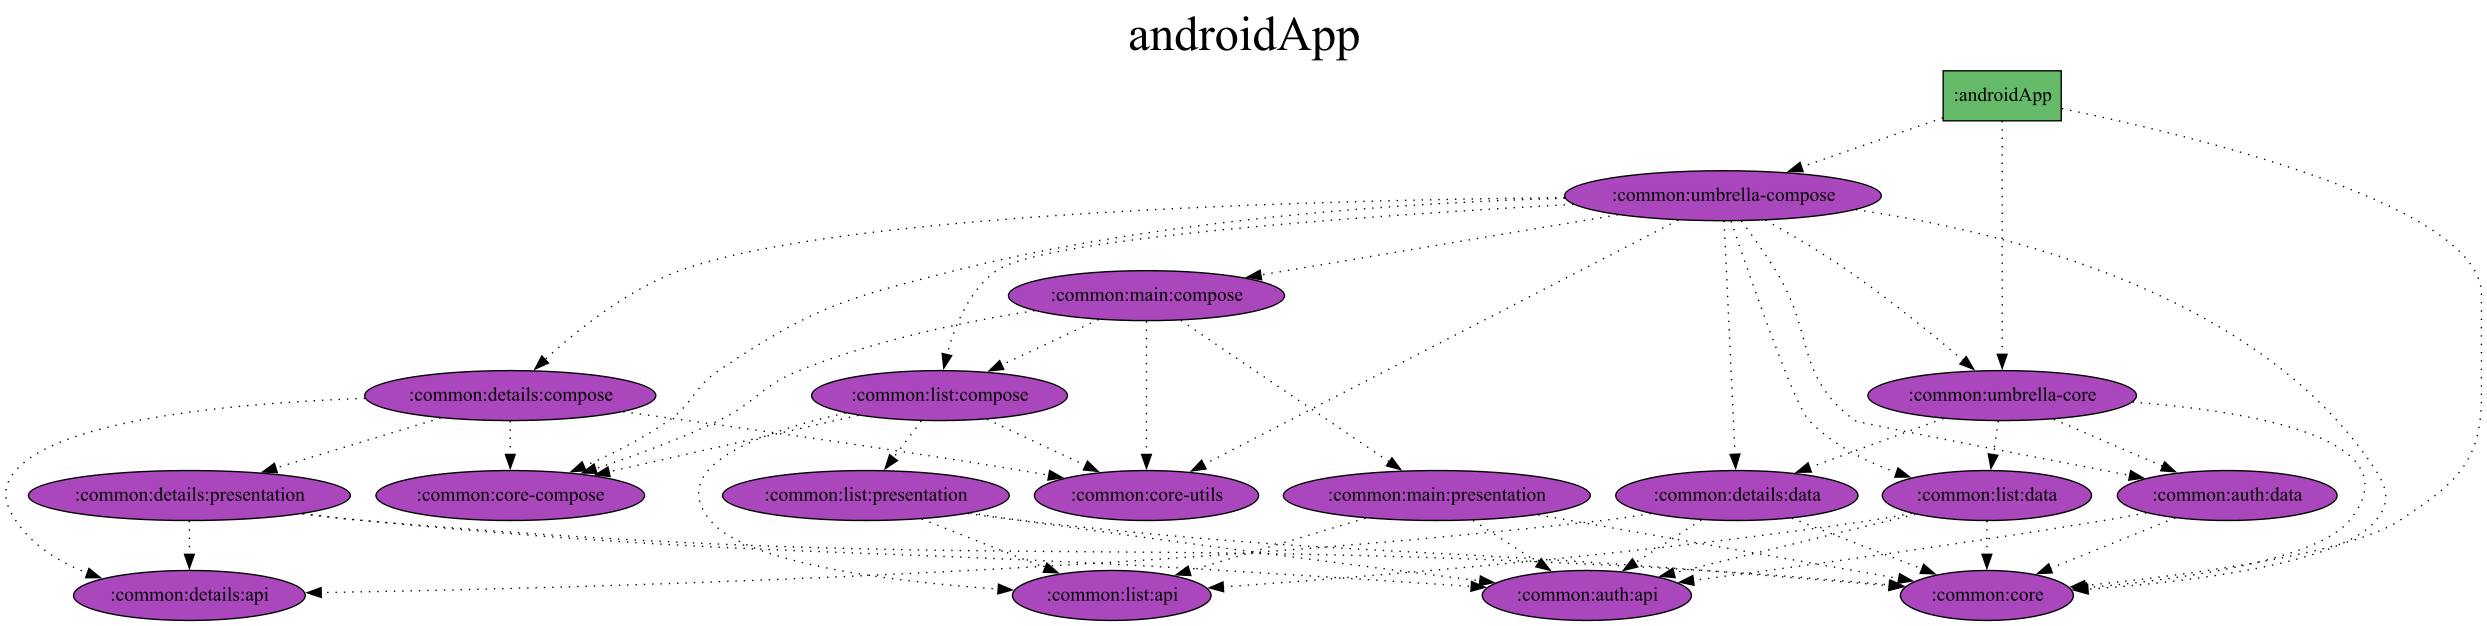
\includegraphics[width=1\textwidth]{Blanks-4LaTeX-main/project-dependency-graph.png}
%\caption{Граф зависимостей проекта.}
%\label{fig:deps-graph}
%\end{figure}

Модуль для пользовательских функциональностей разделены на 4 --- \texttt{api}, \texttt{data}, \texttt{presentation} и \texttt{compose}. В модулях \texttt{api} описываются основные интерфейсы взаимодействия с функциональностью модуля, \texttt{data} --- реализация интерфейсов и дополнительные классы для реализации, \texttt{presentation} --- архитектурная прослойка между пользовательским интерфейсом и \texttt{api}-слоем, о которой будет сказано далее, \texttt{compose} --- реализация графического пользовательского интерфейса функциональности.

Для реализации функциональностей с пользовательским интерфейсом было выбрано использовать архитектурный паттерн \texttt{MVI (Model-View-Intent)}. Данный подход --- один из наиболее популярных \texttt{UDF} паттернов (\texttt{unidirectional data flow} --- однонаправленный поток данных). Существует множество библиотек для реализации данного архитектурного паттерна, для реализации в текущем проекте была выбрана \texttt{KViewModel}~\cite{kvmodel}, имеющая небольшой, но достаточный для реализации \texttt{MVI} набор абстракций. 

Основная сущность данной библиотеки --- абстрактный класс \texttt{BaseViewModel}, принимающий три типа параметров: \texttt{State}, \texttt{Action}, и \texttt{Event}, где \texttt{State} представляет текущее состояние \texttt{View}, \texttt{Action} --- действия, которые могут быть выполнены, и \texttt{Event} --- события, которые приходят от \texttt{View}. Также данный класс имеет публичные методы \texttt{viewStates()} и \texttt{viewActions()}, которые возвращают обёртки над \texttt{StateFlow} и \texttt{SharedFlow} соответственно, что позволяет другим классам подписываться на эти потоки данных, но не менять их и поля \texttt{viewState} и \texttt{viewAction}, которые позволяют получить текущее состояние и действие и установить их новые значения.

Для обработки событий, приходящих от \texttt{View}, данный класс имеет абстрактный метод \texttt{obtainEvent(viewEvent: Event)}, который должен быть реализован в подклассах.

В листинге~\ref{lst:viewmodel-impl} представлен пример реализации \texttt{ViewModel}. В данном классе обрабатываются события, которые приходят с \texttt{View} слоя (\texttt{DelaEvent}), хранится состояние экрана (\texttt{DelaViewState}) и отправляются действия на слой \texttt{View} (\texttt{DelaAction}). \texttt{DelaEvent} и \texttt{DelaAction} представляют собой \texttt{sealed} структуры --- интерфейсы с конечным числом наследников, их код представлен в листинге~\ref{lst:event-action}.

\begin{listing}[!htb]
\caption{Код DelaEvent и DelaAction.}
\label{lst:event-action}
\begin{minted}[frame=single,fontsize = \footnotesize, linenos, xleftmargin = 1.5em, breaklines]{kotlin}
sealed interface DelaAction {
    data class OpenDetails(val id: Int) : DelaAction
}

sealed interface DelaEvent {
    object Refresh : DelaEvent
    object DeloOpen : DelaEvent
    data class DeloClick(val id: Int) : DelaEvent
}
\end{minted}
\end{listing}

События \texttt{DelaAction} отправляются на \texttt{View} слой и обрабатываются там. В листинге~\ref{lst:actions-handling} представден пример обработки данных событий во \texttt{View}. В данном примере из \texttt{ViewModel} приходит событие после нажатия на элемент списка, в результате которого необходимо перейти на экран деталей соответствующего события.

\begin{listing}[!htb]
\caption{Пример обработки Action в View}
\label{lst:actions-handling}
\begin{minted}[frame=single,fontsize = \footnotesize, linenos, xleftmargin = 1.5em,breaklines]{kotlin}
@Composable
fun ListScreen() {
    StoredViewModel(factory = { DelaListViewModel() }) { viewModel ->
        val state = viewModel.viewStates().observeAsState()
        val action = viewModel.viewActions().observeAsState()
        val rootController = LocalRootController.current

        ListView(
            state = state.value,
            onClick = { viewModel.obtainEvent(DelaEvent.DeloClick(it)) }
        )

        when(val action = action.value) {
            is DelaAction.OpenDetails -> {
                val rc = rootController.findRootController()
                rc.present(NavTree.Details.Details.name, params = action.id)
                viewModel.obtainEvent(DelaEvent.DeloOpen)
            }
            null -> {}
        }
    }
}
\end{minted}
\end{listing}

\subsection{Итоговое описание приложения}

В результате работы было разработано клиентское приложение, имеющее общий код на Kotlin, использующее HTTP и Rest Api для сетевого взаимодействия и сохраняющее данные локально.

Для сетевых запросов на предоставленном API используется Bearer аутенфикация, в связи с чем необходимо сохранять токен для HTTP запросов. Однако, не реализован механизм для Refresh токенов, из-за чего перед каждым сетевым запросом необходимо проверять текущий сохранённый токен на валидность. В случае истечения срока действия токена, повторно отправляется запрос авторизации с сохранёнными данными для входа, вследствии чего обновляется токен.

На главном экране приложения выводится список Новомученников на текущий день. Все данные, получаемые по запросу на главном экране, сохраняются в базе данных. В случае отсутствия интернета выводятся список из всех сохранённых ранее данных, вне зависимости от даты.

При нажатии на элемент списка отправляется запрос на получение деталей про конкретного человека. Предварительно проверяется валидности токена, как уже было сказано ранее. На экране деталей выводятся фамилия, имя и отчество новомученника, дата смерти и ключевые записанные события из базы данных электронно биографического справочника собранного на основе базы данных <<За Христа пострадавшие>>.

\section{Тестирование приложения}\label{sect:testing}

В данной главе будет описано тестирование сборки приложений с использованием инструментов Github Actions. Также будет представлен результат запуска приложения на платформах iOS, Android и Desktop

\subsection{Проверка сборки в Github Actions}

Для управления версиями данного проекта используется сервис Github. Благодаря использованию этого сервиса, возможно автоматизировать некоторые процессы, связанные с проектом. Например, возможно использовать Github Actions для автоматического запуска определенных задач при отправке нового кода. Для проверки сборки и распространения сборок в Telegram было реализовано несколько пайплайнов.

Когда происходят изменения в рамках Pull Request или коммит в одну из главных веток (dev, master), происходит автоматическая сборка проекта Android и загрузка \texttt{.apk} файла в канал Telegram (debug-сборка для Pull Request, release --- для dev и master). Также запускается сборка Desktop-приложения без отправки артефакта, для проверки сборки. Обе сборки запускаются с помощью gradle задачи. Однако, чтобы выполнить сборку iOS-проекта, необходимо выполнить дополнительные шаги, из-за чего сборка iOS на CI не производится.

В листинге~\ref{lst:android-pr} представлен код для сборки Android приложения на Pull Request в главные ветки (\texttt{dev} и \texttt{master}). Сборка Desktop-приложения производится по аналогии, однако из кода удалены части, отвечающие за создание версии и загрузку файла в Telegram. Также аналогичным образом реализована сборка и загрузка приложений из веток \texttt{dev} и \texttt{master}.

На рисунке~\ref{fig:tg-upload} представлен пример загрузки приложения в Telegram-канал. По аналогии возможно настроить загрузку приложения в любой другой источник, включая загрузку сразу в магазины приложений для распространения новых версий.

\subsection{Снимка экранов страниц под iOS Android Desktop}

На рисунках~\ref{fig:run},~\ref{fig:run2} представлен результат запуска приложения на платформах iOS, Android, Desktop.

\begin{figure}[!htb]
\centering
  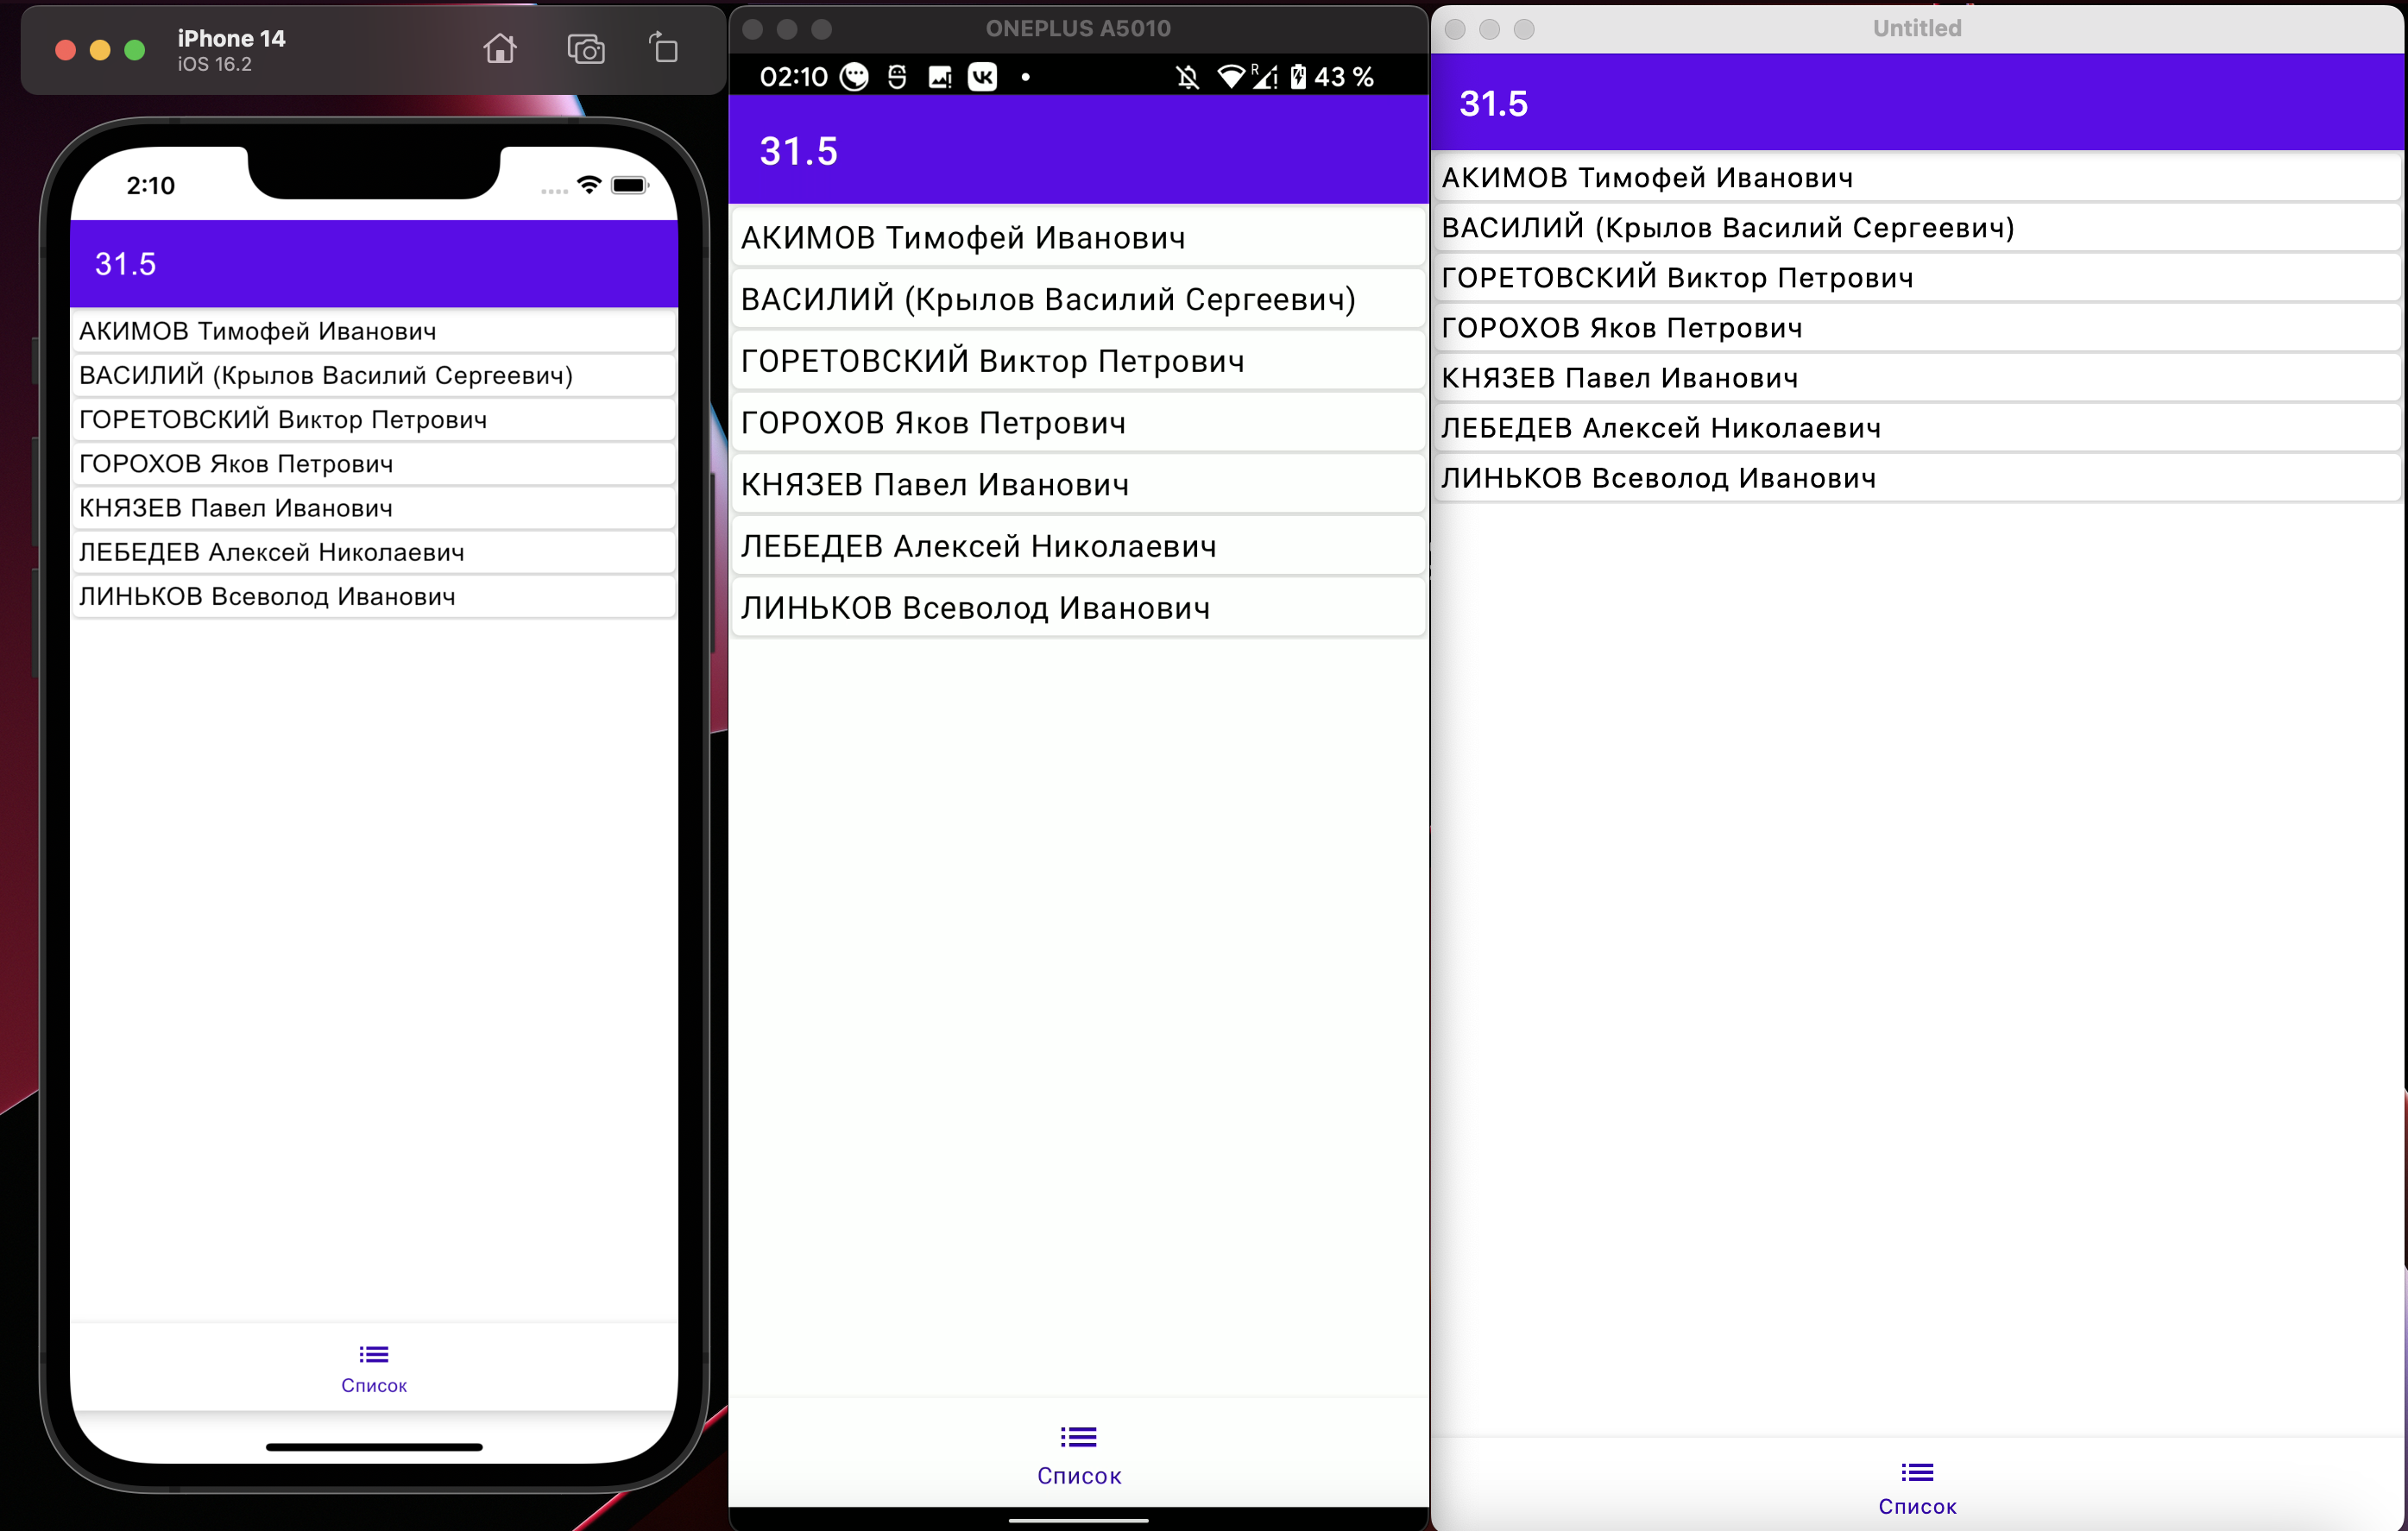
\includegraphics[width=0.75\textwidth]{Blanks-4LaTeX-main/run.png}
\caption{Экран списка на iOS, Android, Desktop}
\label{fig:run}
\end{figure}

\begin{figure}[!htb]
\centering
  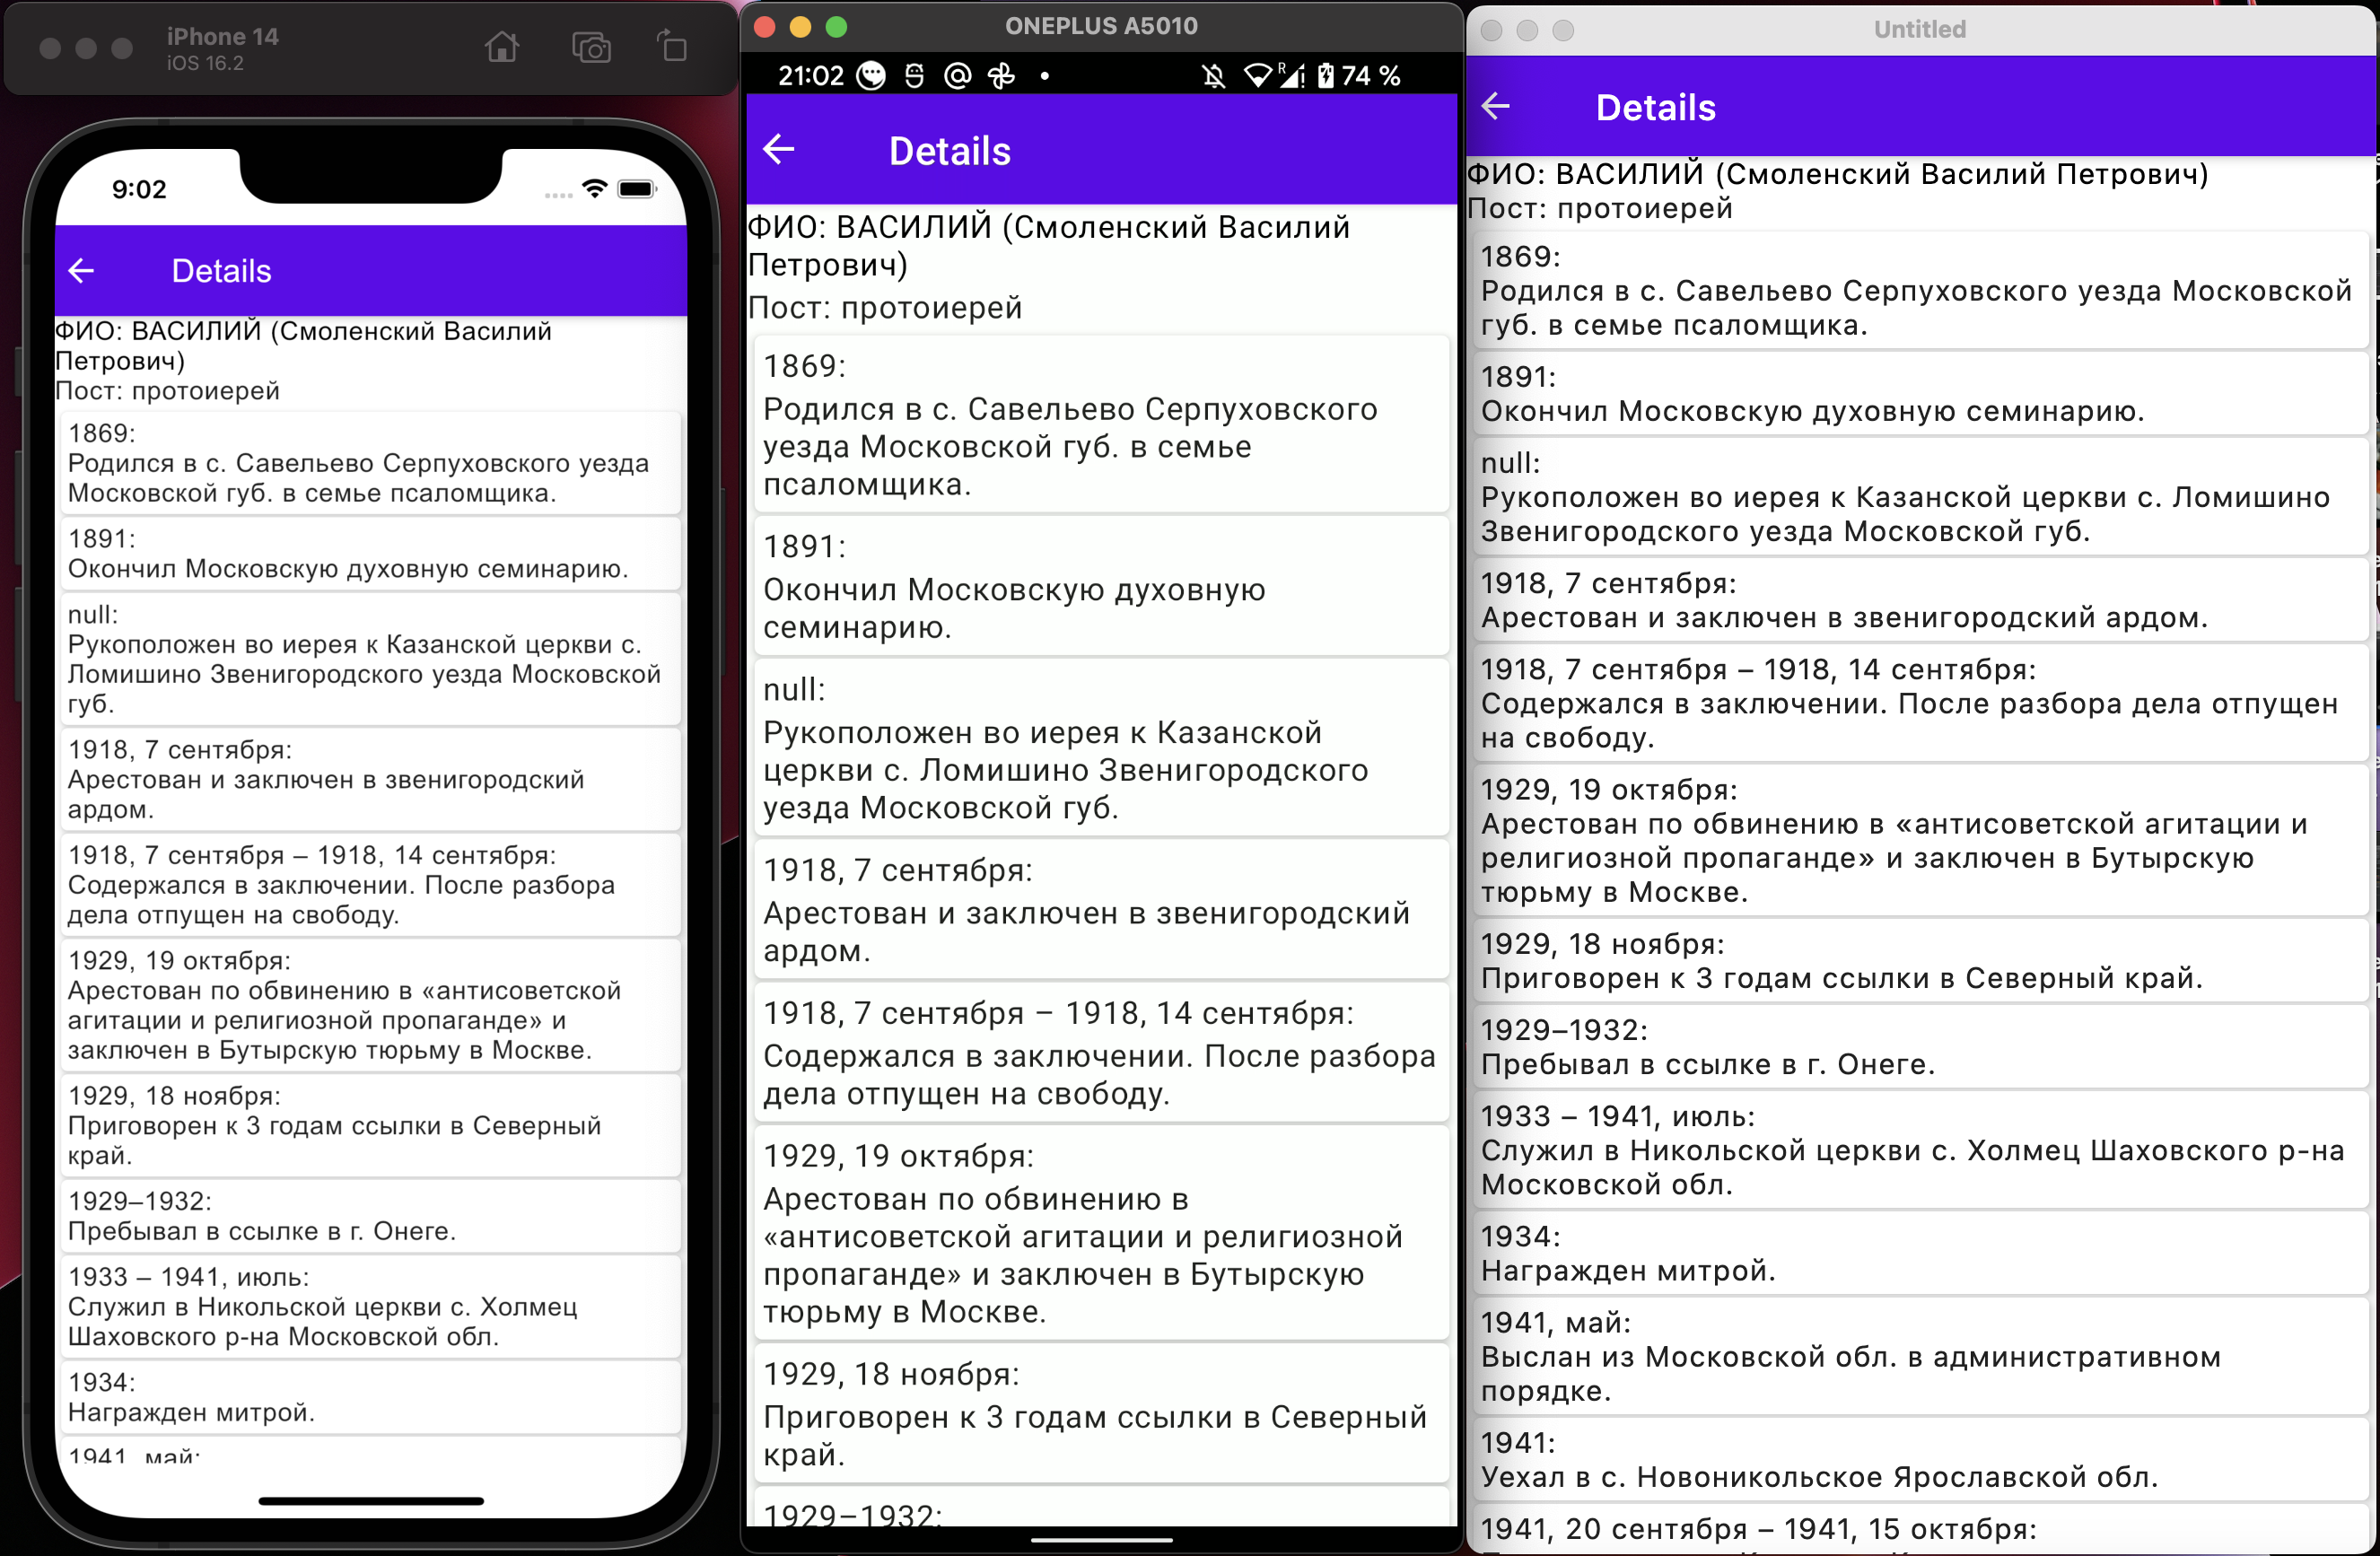
\includegraphics[width=0.75\textwidth]{Blanks-4LaTeX-main/Screenshot 2023-06-12 at 21.02.20.png}
\caption{Экран деталей на iOS, Android, Desktop}
\label{fig:run2}
\end{figure}

\anonsection{ЗАКЛЮЧЕНИЕ} 

В данной работе был произведён детальный обзор мультиплатформенной разработки и сравнение различных технологий в этой области, таких как нативная разработка, Xamarin, React Native, Flutter и Kotlin Multiplatform. В результате анализа в качестве наиболее подходящей технологии для данного исследования был выбран Kotlin Multiplatform.

Были раскрыты преимущества Kotlin Multiplatform, включая поддержку различных платформ (JVM/Android, Native, JS и WebAssembly) и особенности компиляции под разные целевые платформы. Данный подход позволяет максимально использовать преимущества разработки на одном языке и обеспечивает высокую производительность и кросс-платформенность приложений.

Был произведён разбор процесса разработки приложения, включая настройку проекта, выбор и подключение библиотек, использование convention plugins, организацию общего и платформенного кода. Важно отметить использование механизма "ожидание-актуализация" (expect-actual), который позволяет более гибко управлять разработкой для различных платформ.

На практике было демонстрировано написание общего кода, включая настройку DI в проекте, сетевые запросы с помощью Ktor, использование SQLDelight для работы с базой данных, создание графического пользовательского интерфейса с навигацией, сохранение простых данных, а также была описана архитектура приложения.

Итак, данная работа подтвердила эффективность Kotlin Multiplatform для разработки мультиплатформенных приложений.


\renewcommand\refname{СПИСОК ИСПОЛЬЗОВАННЫХ ИСТОЧНИКОВ}
% Список литературы
\clearpage
%\bibliographystyle{ugost2008s}  %utf8gost71u.bst} %utf8gost705u} %gost2008s}
{\catcode`"\active\def"{\relax}
\addcontentsline{toc}{section}{\protect\numberline{}\refname}%
%\bibliography{biblio} %здесь ничего не меняем, кроме, возможно, имени bib-файла
\printbibliography
}
\newpage
\settocdepth{section}

\anonsection{ПРИЛОЖЕНИЕ А}\label{sect:appl-a}

\vspace{-20pt}

\begin{longlisting}
\caption{Файл build.gradle.kts umbrella модуля.}
\label{lst:umbrella-build-gradle}
\begin{minted}[frame=single,fontsize = \footnotesize, linenos, xleftmargin = 1.5em,breaklines]{kotlin}
plugins {
    id("mp-compose-setup")
    id("android-setup")
    kotlin("native.cocoapods")
}
version = "0.0.1"
kotlin {
    cocoapods {
        summary = "MPP iOS SDK + Compose"
        homepage = "https://google.com"
        ios.deploymentTarget = "14.0"
        podfile = project.file("../../apps/iosApp/Podfile")
        framework {
            transitiveExport = false
            isStatic = true
            baseName = "shared_compose"
            freeCompilerArgs += "-Xbinary=bundleId=ru.andvl.mppapp"
            export(projects.common.core)
            export(projects.common.coreUtils)
            export(projects.common.coreCompose)
            export(projects.common.auth.data)
            export(projects.common.main.compose)
            export(projects.common.list.data)
            export(projects.common.list.compose)
            export(projects.common.umbrellaCore)
        }
    }
    sourceSets {
        commonMain {
            dependencies {
                implementation(projects.common.core)
                implementation(projects.common.coreUtils)
                implementation(projects.common.coreCompose)

                implementation(projects.common.auth.data)

                implementation(projects.common.main.compose)

                implementation(projects.common.list.data)
                implementation(projects.common.list.compose)

                implementation(projects.common.umbrellaCore)

                implementation(libs.kViewModel.core)
                implementation(libs.kViewModel.compose)
                implementation(libs.kViewModel.odyssey)

                implementation(libs.odyssey.core)
                implementation(libs.odyssey.compose)
            }
        }
        androidMain {
            dependencies {
                implementation(project.dependencies.platform(
                    libs.androidx.compose.bom
                ))
                implementation(libs.compose.activity)
            }
        }
        iosMain {
            dependencies {
                api(projects.common.core)
                api(projects.common.coreUtils)
                api(projects.common.coreCompose)
                api(projects.common.auth.data)
                api(projects.common.main.compose)
                api(projects.common.list.data)
                api(projects.common.list.compose)
                api(projects.common.umbrellaCore)
            }
        }
    }
}
\end{minted}
\end{longlisting}

\newpage
\settocdepth{section}

\anonsection{ПРИЛОЖЕНИЕ Б}\label{sect:appl-b}

\vspace{-20pt}

\begin{longlisting}
\caption{Convention plugin для модулей с графическим пользовательским интерфейсом.}
\label{lst:compose-convention}
\begin{minted}[frame=single,fontsize = \footnotesize, linenos, xleftmargin = 1.5em,breaklines]{kotlin}
plugins {
    id("com.android.library")
    kotlin("multiplatform")
    id("org.jetbrains.compose")
}

kotlin {
    jvm("desktop")
    android()
    ios()
    iosSimulatorArm64()

    sourceSets {
        val iosSimulatorArm64Main by getting
        val iosSimulatorArm64Test by getting
        val commonMain by getting {
            dependencies {
                implementation(compose.runtime)
                implementation(compose.foundation)
                implementation(compose.material)
                implementation(compose.ui)
            }
        }

        named("desktopMain") {
            dependencies {
                implementation(compose.desktop.common)
            }
        }

        named("androidMain") {
            dependencies {
                implementation(project.dependencies.platform(
                    libs.androidx.compose.bom
                ))
                implementation(libs.compose.ui)
                implementation(libs.compose.material)
                implementation(libs.compose.tooling)
                implementation(libs.compose.icons)
            }
        }
        val iosMain by getting {
            dependsOn(commonMain)
            iosSimulatorArm64Main.dependsOn(this)
        }
        val iosTest by getting  {
            dependsOn(commonMain)
            iosSimulatorArm64Test.dependsOn(this)
        }
    }

    tasks.withType<org.jetbrains.kotlin.gradle.tasks.KotlinCompile> {
        kotlinOptions.jvmTarget = "11"
    }
}
\end{minted}
\end{longlisting}

\anonsection{ПРИЛОЖЕНИЕ В}\label{sect:appl-v}

\vspace{-20pt}

\begin{figure}[!htb]
\centering
  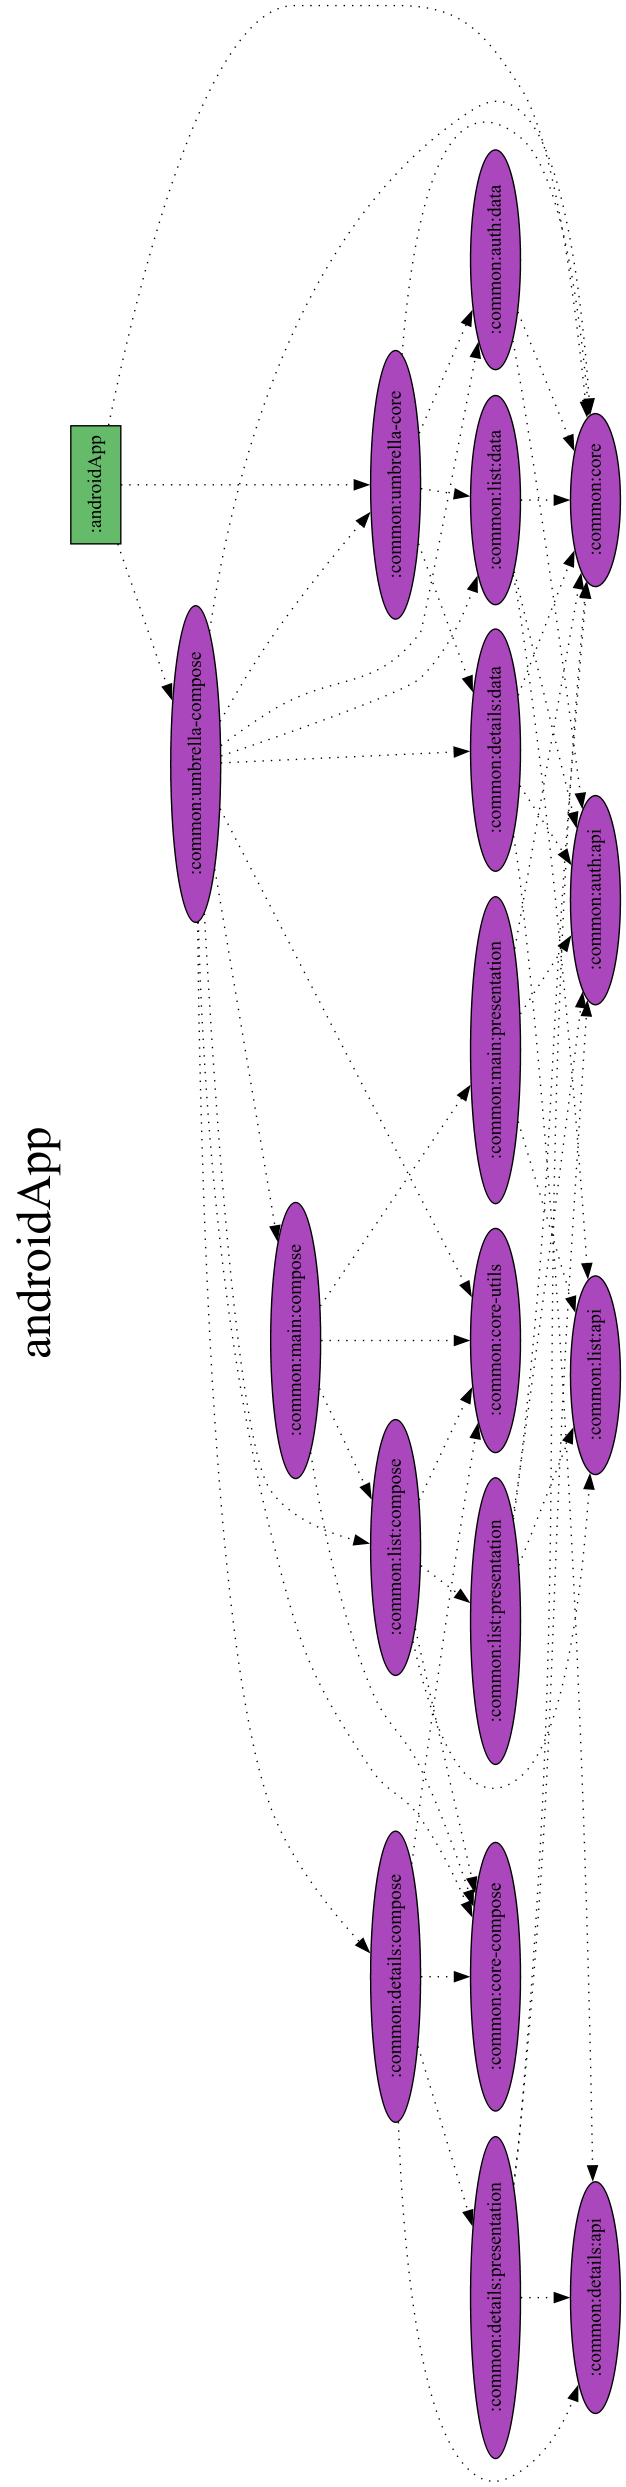
\includegraphics[width=0.33\textwidth]{Blanks-4LaTeX-main/project-dependency-graph-2.png}
\caption{Граф зависимостей проекта.}
\label{fig:deps-graph2}
\end{figure}

\anonsection{ПРИЛОЖЕНИЕ Г}\label{sect:appl-g}

\vspace{-20pt}

\begin{figure}[!htb]
\centering
  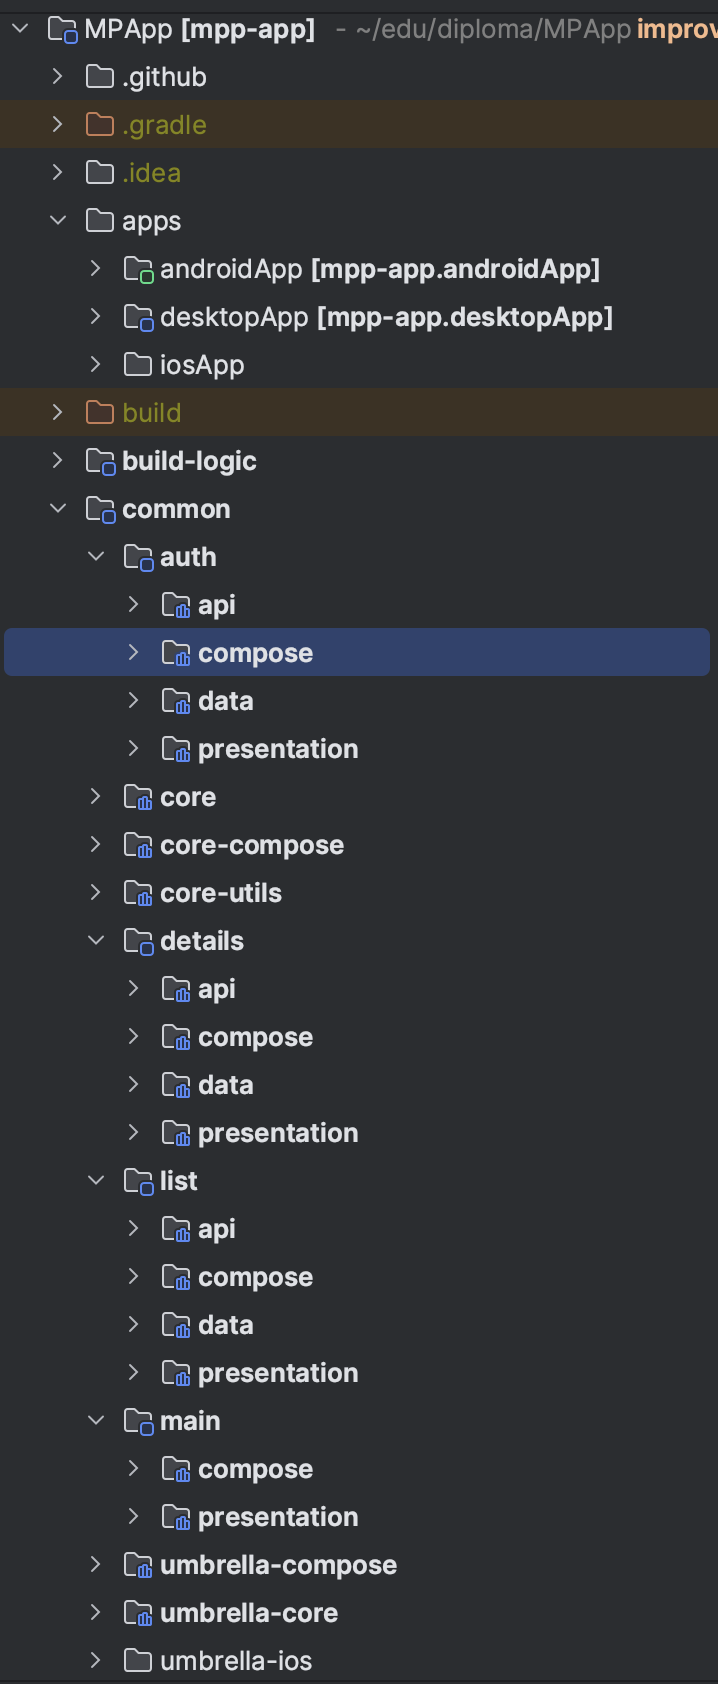
\includegraphics[width=0.5\textwidth]{Blanks-4LaTeX-main/structure.png}
\caption{Структура проекта.}
\label{fig:project-structure}
\end{figure}

\anonsection{ПРИЛОЖЕНИЕ Д}\label{sect:appl-d}

\vspace{-20pt}

\begin{longlisting}
\caption{Пример реализации ViewModel.}
\label{lst:viewmodel-impl}
\begin{minted}[frame=single,fontsize = \footnotesize, linenos, xleftmargin = 1.5em,breaklines]{kotlin}
class DelaListViewModel : BaseSharedViewModel<DelaViewState, DelaAction, DelaEvent>(
    initialState = DelaViewState()
) {
    private val authRepository: AuthRepository = Inject.instance()
    private val delaRepository: DelaListRepository = Inject.instance()

    init {
        viewModelScope.launch {
            viewState = viewState.copy(isLoading = true)
            checkLogin()
            getDela()
        }
    }

    override fun obtainEvent(viewEvent: DelaEvent) {
        when (viewEvent) {
            is DelaEvent.Refresh -> {
                viewState = viewState.copy(isLoading = true, dela = null, isError = false)
                viewModelScope.launch {
                    getDela()
                }
            }
            is DelaEvent.DeloClick -> {
                viewAction = DelaAction.OpenDetails(viewEvent.id)
            }
            is DelaEvent.DeloOpen -> {
                viewAction = null
            }
        }
    }

    private suspend fun checkLogin() {
        // поход в authRepository для проверки авторизации пользователя
    }

    private suspend fun getDela() {
        val now = Clock.System.now()
        val datetime = now.toLocalDateTime(TimeZone.currentSystemDefault())
        val dela = delaRepository.getDelas(token = authRepository.getToken())
        viewState = if (dela != null) {
            viewState.copy(
                isLoading = false,
                dela = dela,
                date = "${datetime.dayOfMonth}.${datetime.monthNumber}"
            )
        } else {
            viewState.copy(isLoading = false, isError = true)
        }
    }
}
\end{minted}
\end{longlisting}

\anonsection{ПРИЛОЖЕНИЕ Е}\label{sect:appl-e}

\vspace{-20pt}

\begin{longlisting}
\caption{Сборка Android приложения на Pull Request.}
\label{lst:android-pr}
\begin{minted}[frame=single,fontsize = \footnotesize, linenos, xleftmargin = 1.5em,breaklines]{yaml}
name: Build Android Pull request

on:
  pull_request:
    branches:
      - 'dev'
      - 'master'

env:
  GITHUB_REF: github.ref

jobs:
  build:
    name: "Build apk"
    runs-on: ubuntu-latest
    outputs:
      build_number: ${{ steps.buildnumber.outputs.build_number }}
    steps:
      - uses: actions/checkout@v2
        with:
          submodules: 'recursive'
      - name: Set up JDK 1.11
        uses: actions/setup-java@v2
        with:
          distribution: 'temurin'
          java-version: '11'
      - name: Generate build number
        id: buildnumber
        uses: onyxmueller/build-tag-number@v1
        with:
          token: ${{secrets.github_token}}

      - name: Gradle Wrapper Validation
        uses: gradle/wrapper-validation-action@v1

      - uses: actions/cache@v2
        with:
          path: |
            ~/.gradle/caches
            ~/.gradle/wrapper
          key: ${{ runner.os }}-gradle-${{ hashFiles('**/*.gradle*', '**/gradle-wrapper.properties') }}
          restore-keys: |
            ${{ runner.os }}-gradle-
      - name: 'Set variables'
        id: vars
        run: |
          export $(cat .github/workflows/version.env | xargs)
          echo "::set-output name=major_version::${MAJOR_VERSION}"
          echo ${{ steps.buildnumber.outputs.build_number }} > version.txt
      - name: Build dev
        run: |
          ./gradlew generateCommonMainDatabaseInterface :androidApp:assembleDebug \
            -Dversion_code=${{ steps.buildnumber.outputs.build_number }} \
            -Dversion_name="${{ steps.vars.outputs.major_version }}" \
      - name: Copy artifacts
        id: artifacts_copy
        run: |
          mkdir artifacts
          cp version.txt artifacts/version.txt
          cp apps/androidApp/build/outputs/apk/debug/androidApp-debug.apk artifacts/app-debug-`cat version.txt`.apk
          echo "::set-output name=path::artifacts/"
      - name: Upload Artifacts
        uses: actions/upload-artifact@v2
        with:
          name: artifacts
          path: ${{ steps.artifacts_copy.outputs.path }}
  upload-to-tg:
    name: Upload to tg channel
    runs-on: ubuntu-latest
    needs: build
    steps:
      - uses: actions/checkout@v2
      - uses: actions/download-artifact@v2
        id: download
        with:
          name: artifacts
      - name: Get version number
        id: version-num
        run: |
          echo "::set-output name=num::`cat ${{steps.download.outputs.download-path}}/version.txt`"
      - name: Upload to Telegram
        uses: appleboy/telegram-action@master
        with:
          to: ${{ secrets.TELEGRAM_TO }}
          token: ${{ secrets.TELEGRAM_TOKEN }}
          message: |
            New commit in pull request #${{ github.event.pull_request.number }}: ${{ github.event.pull_request.title }}
            View: https://github.com/AndVl1/mpp-diploma-app/pull/${{ github.event.pull_request.number }}
          document: ${{ steps.download.outputs.download-path }}/app-debug-${{ steps.version-num.outputs.num }}.apk
          disable_notification: true

\end{minted}
\end{longlisting}

\anonsection{ПРИЛОЖЕНИЕ Ж}\label{sect:appl-j}

\vspace{-20pt}

\begin{figure}[!htb]
\centering
  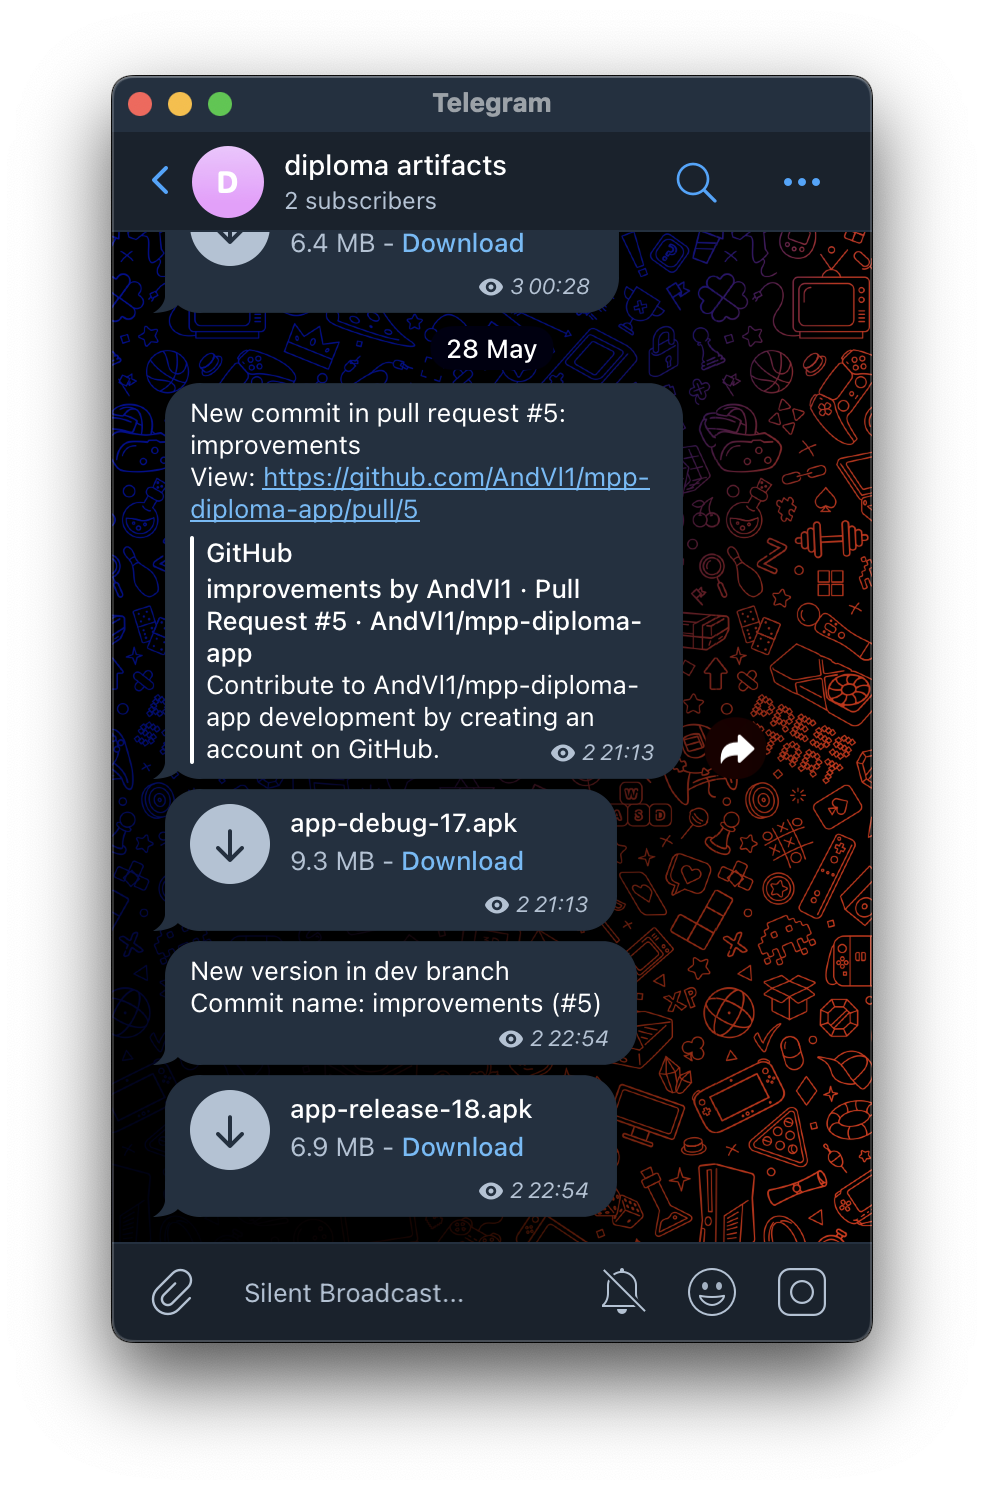
\includegraphics[width=0.5\textwidth]{Blanks-4LaTeX-main/Screenshot 2023-05-29 at 00.22.39.png}
\caption{Пример загруженных в Telegram Android приложений из Pull Request и из ветки dev.}
\label{fig:tg-upload}
\end{figure}

\end{document}
